\documentclass[11pt,a4paper]{article}

% Define page geometry
\usepackage{geometry}
\geometry{left=2.2cm,
	right=2.2cm,
	top=2.2cm,
	bottom=2cm}
\parskip 0.15cm
\setlength{\parindent}{0cm}
\usepackage{pdflscape}
\usepackage[document]{ragged2e}

% Set font
\usepackage[T1]{fontenc}

% Image handling
\usepackage{graphics}  % Insert images easily
\usepackage{graphicx}  % Extended image support

\makeatletter
	\g@addto@macro\@floatboxreset\centering  % Automatically centre images (floats)
\makeatother

\graphicspath{ {img/} }
\usepackage{float}  %  Graphics placement [H] [H!] arguments
\usepackage{subfig}  % Compound figures

% Tables
\usepackage{multirow}
\usepackage{longtable}

% Bibliography management
\usepackage{natbib}    % Bibliography management - Use author/date citations
\bibliographystyle{agsmnourl}  % Use custom agsm bibliography template with no URL
\usepackage{cite}  % Citation options

% Text formatting
\usepackage{url} % Allow nice formatting of URLs in text

\usepackage{enumerate}  % Enumerated lists

\usepackage{lineno}  % Line numbers

\usepackage{textcomp}
\newcommand{\textapprox}{\raisebox{0.5ex}{\texttildelow}}  % Command for a good tilde

\usepackage{siunitx}
\usepackage{amsmath}

\usepackage{xcolor}
\newcommand{\todo}[1]{\textcolor{red}{\textbf{#1}}}   % \todo{NOTE TO SELF WRITTEN IN RED}

\usepackage[revision]{revdiff}


\input{code_format}

% Custom title formatting
\let\oldtitle\title

\renewcommand{\title}[1]{\oldtitle{\vspace{-1.5cm}#1}}

\usepackage[breaklinks]{hyperref}
\definecolor{links}{RGB}{191,59,72}
\hypersetup{
	breaklinks,
	colorlinks,
	allcolors=links,
	linktoc=section,
	pdfauthor={John L. Godlee}
}
\def\subsectionautorefname{section}
\def\subsubsectionautorefname{section}
% \usepackage{biblatex}

\usepackage{dcolumn}
\usepackage{multirow}
\usepackage{tikz}
\usetikzlibrary{calc,arrows,positioning,shapes,shapes.gates.logic.US,trees}
\usepackage{pdflscape}
\usepackage{longtable}
\usepackage{fmtcount}

\usepackage{lineno}
\linenumbers

\title{An assessment of the biodiversity - ecosystem function relationship in southern African woodlands}
\author{}
\date{}

\newcommand{\nplots}{1767}
\newcommand{\nplotspcoa}{1877}
\newcommand{\nstems}{93242}

\newcommand{\noutliers}{76}

\newcommand{\hullcover}{94.4}

\newcommand{\pcsdsd}{1}
\newcommand{\pcsded}{1.03}
\newcommand{\pcshdh}{1}
\newcommand{\pcshhh}{0.73}
\newcommand{\pcsdb}{-0.14}
\newcommand{\pcshb}{0.41}
\newcommand{\pcsdh}{0.42}
\newcommand{\pcsib}{0.77}
\newcommand{\pcsdi}{0.17}
\newcommand{\strucrsq}{0.7}
\newcommand{\strucbrsq}{0.69}
\newcommand{\struccrsq}{0.72}
\newcommand{\strucsib}{$\beta =$ NA$\pm$NA, p = NA}
\newcommand{\strucbsb}{$\beta =$ -0.25$\pm$0.064, p <0.01}
\newcommand{\strucbhb}{$\beta =$ 0.28$\pm$0.049, p <0.01}
\newcommand{\struccsb}{$\beta =$ 0.14$\pm$0.118, p = 0.24}

\newcommand{\rgmbd}{$\beta =$ 0.02$\pm$0.008, p = 0.06}
\newcommand{\rgsbd}{$\beta =$ 0.02$\pm$0.008, p = 0.05}
\newcommand{\rgid}{$\beta =$ 0.62$\pm$0.034, p <0.01}
\newcommand{\rghb}{$\beta =$ 0.33$\pm$0.042, p <0.01}
\newcommand{\fmrsq}{0.5}
\newcommand{\fmrmsea}{0.166}
\newcommand{\fmtli}{0.905}
\newcommand{\fmcfi}{0.924}
\newcommand{\pcfmmp}{1}
\newcommand{\pcfmmpc}{0.11}
\newcommand{\pcfmmt}{0.17}
\newcommand{\pcfmmtc}{0.57}
\newcommand{\pcfdds}{1}
\newcommand{\pcfdde}{0.72}
\newcommand{\pcfsss}{1}
\newcommand{\pcfsso}{0.31}
\newcommand{\pcfssc}{0.37}
\newcommand{\pcfhhh}{1}
\newcommand{\pcfhhd}{0.96}
\newcommand{\pcfmd}{0.21}
\newcommand{\pcfsd}{0.21}
\newcommand{\pcfdh}{0.3}
\newcommand{\pcfmi}{-0.01}
\newcommand{\pcfsi}{-0.01}
\newcommand{\pcfdi}{0.62}
\newcommand{\pcfsb}{0.03}
\newcommand{\pcfmb}{0.01}
\newcommand{\pcfdb}{0.07}
\newcommand{\pcfhb}{0.33}
\newcommand{\pcfib}{0.49}
\newcommand{\srsq}{46}

\newcommand{\ccib}{$\rho =$ 0.78, p <0.01}
\newcommand{\ccmb}{$\rho =$ 0.24, p <0.01}
\newcommand{\ccmcb}{$\rho =$ -0.09, p <0.01}
\newcommand{\ccob}{$\rho =$ 0.23, p <0.01}
\newcommand{\ccsb}{$\rho =$ -0.25, p <0.01}
\newcommand{\ccms}{$\rho =$ 0.39, p <0.01}
\newcommand{\ccme}{$\rho =$ 0.1, p <0.01}
\newcommand{\ccmh}{$\rho =$ 0.21, p <0.01}
\newcommand{\ccmi}{$\rho =$ 0.12, p <0.01}
\newcommand{\ccsi}{$\rho =$ 0.54, p <0.01}
\newcommand{\ccei}{$\rho =$ 0.47, p <0.01}
\newcommand{\cctb}{$\rho =$ -0.05, p <0.05}
\newcommand{\cctcb}{$\rho =$ -0.19, p <0.01}

\newcommand{\moderp}{$\beta =$ 0, t(1765) = 0.19, p = 0.85}
\newcommand{\moders}{$\beta =$ 0.02, t(1765) = 0.89, p = 0.38}

\newcommand{\subn}{80}
\newcommand{\subp}{359.4}

\newcommand{\percsmallagb}{2.1}


\begin{document}

{\LARGE{Title: An assessment of the biodiversity - ecosystem function relationship in southern African woodlands}}

\vspace{1cm}

Authors: Godlee, J. L.\textsuperscript{1}, Dexter, K. G.\textsuperscript{1}, Ryan, C. M.\textsuperscript{1}

\textsuperscript{1}: School of GeoSciences, University of Edinburgh, Edinburgh, United Kingdom \\
\textsuperscript{2}: Some other address

\vspace{1em}
Corresponding author:

John L. Godlee

johngodlee@gmail.com

School of GeoSciences, University of Edinburgh, Edinburgh, United Kingdom


\section*{Acknowledgements}

This work is funded by a NERC E3 Doctoral Training Partnership PhD studentship at the University of Edinburgh (J. L. Godlee, Grant No. NE/L002558/1). The data provided for this study was constributed by a number of independently funded projects and was assembled and prepared by SEOSAW (A Socio-Ecological Observatory for Southern African Woodlands), an activity of the Miombo Network and NERC-funded project (Grant No. NE/P008755/1). We thank all data providers and the field assistance they received when collecting plot data. 

\section*{Biosketch}

SEOSAW (A Socio-Ecological Observatory for Southern African Woodlands, \url{https://seosaw.github.io}) aims to understand the response of southern African woodlands to global change. The goal of SEOSAW is to produce novel analyses of the determinants of ecosystem structure and function for the southern Africa region, based on syntheses of plot data. Additionally the group hopes to develop infrastructure for a long-term regional plan for plot remeasurement in the southern African region. While working on a multitude of diverse projects in the dry tropics at large, all authors have a broad interest in community ecology and ecosystem assemblage in southern African woodlands.

\newpage{}

{\LARGE{\textbf{Blinded Main Text File}}}

\LARGE{Title: An assessment of the biodiversity - ecosystem function relationship in southern African woodlands}

\normalsize{Running title: Ecosystem function in southern African woodlands}

\section*{Abstract}

\textbf{Aim:} Positive correlations between tree biodiversity and ecosystem function have been widely documented, but the nature of the relationship \rchange{in highly disturbed and ecophysiologically stressful systems is less clear}{in southern African savanna/woodlands, which experience high levels of disturbance and ecophysiological stress, is less clear}. Here, we explore the relationship between tree biodiversity and aboveground biomass across southern African savannas and woodlands, with respect to gradients in stem density, resource availability \rnew{and disturbance through fire}, to build a general understanding of the biodiversity - ecosystem function relationship in this understudied ecological context.

\textbf{Location:} Southern African savannas and woodlands

\textbf{Time period:} 2010-2019

\textbf{Major taxa studied:} Trees

\textbf{Methods:} We used a network of \nplots{} savanna/woodland plots located across the southern African sub-continent in which each tree >10 cm diameter was measured \rnew{and identified to species level}. We used structural equation modelling and path analysis to determine the relationship between tree species diversity and aboveground woody biomass, accounting for the interactive effects of resource availability and along a gradient of stem density.

\textbf{Results:} A positive effect of tree species diversity on aboveground biomass was demonstrated, observed largely as an indirect effect of increasing woodland structural diversity. We also found that the effect of tree species diversity on biomass increases with stem density. Finally, we found that resource availability affects biomass in southern African woodlands largely indirectly via its effect on species diversity.

\textbf{Main conclusions:} The study underlines the close association between tree diversity, ecosystem structure and function of highly disturbed southern African savannas and woodlands. Our results demonstrate the importance of including environmental conditions and vegetation type in models to accurately describe a general relationship between biodiversity and ecosystem function at a regional level. Biodiversity loss predominantly by human actions in southern Africa may have detrimental outcomes for ecosystem function, particularly in species poor Baikiaea woodlands, which showed the strongest biodiversity - ecosystem function relationship.

% Studies in natural and experimental settings have shown a positive relationship between tree species diversity and ecosystem functionality but many ecosystems are understudied in this regard. In this study we conducted the first regional estimation of the relationship between tree species diversity and above-ground biomass in southern African woodlands, using a network of \nplots{} woodland plots. We used structural equation modelling (SEM) to determine the relationship between tree species diversity and aboveground biomass, with comparison to the effects of resource availability and along a gradient of stem density. A positive effect of tree species diversity on biomass was demonstrated, with most of this as an indirect effect via woodland structural diversity. We found that the effect of tree species diversity on biomass increases with stem density. Finally, we found that resource availability determines biomass in southern African woodlands largely indirectly via its effect on species diversity.

\section*{Introduction}

Scientific interest in the relationship between species richness and ecosystem function springs from both an interest in the factors which structure ecological communities \citep{}, and a more applied interest in determining the effect of global biodiversity loss on ecosystem form and function \citep{}. Numerous studies have shown relationships between biodiversity and ecosystem function (e.g. \citealt{Liang2016, Hooper2012, Cardinale2009}). The strength and direction of these observed Biodiversity-Ecosystem Function Relationships (BEFRs) varies depending on the ecosystem being studied, the ecosystem function(s) of interest \citep{Hector2007}, and the inclusion of environmental covariates in statistical models \citep{Vila2005}, but there appears to be a generalisable positive correlation between biodiversity and ecosystem function \citep{Liang2016}. Over the past decade, many observational studies of the BEFR have been conducted, mostly in wet tropical and temperate forests, and grasslands \citep{Chen2011}. These studies support early findings from small scale experimental studies predominantly in grassland patches, which began in earnest during the 1990s as concern grew over the global loss of biodiversity \citep{Tilman1994, Tilman2014}.

Ecosystem functions can be defined in broad terms as rate processes and properties of ecosystems which describe the degree of biotic activity within an ecosystem \citep{Jax2005}. This includes basic processes of primary production such as gross primary productivity and atmospheric nitrogen fixation, but can be extended to indirect measures of function such as resistance of productivity to disturbance, and further to ecosystem properties which themselves influence process, such as trophic complexity and total vegetative biomass. The frequently reported and intuitive relationship between biodiversity and ecosystem function invokes three main mechanisms which drive the relationship \citep{Tilman2014}: 1) niche complementarity, whereby communities with greater diversity fill a greater breadth of realised niche space and avoid competition due to differences in their traits, 2) selection effects, whereby communities with greater diversity are more likely to include a species which contributes highly to the measured ecosystem function, and 3) facilitation effects, whereby communities with greater diversity are more likely to include combinations of species which together increase the others' functional contribution.

Compared to \rchange{other forested}{forest} ecosystems, dry tropical woodlands and savannas are highly structured by disturbance, mainly through fire \rchange{and in Africa notably by herbivory also}{and herbivory, with African savannas possessing large herbivores absent from other savannas} \citep{Sankaran2008, Levick2009}. \rnew{Disturbance via human activities such as timber extraction and charcoal processing is also common in African woodlands, often causing high levels of disturbance in localised areas \citep{}}. High levels of disturbance may weaken the role of competition in determinging local species distribution and allow weak competitors to co-exist where they would normally be excluded \citep{Grime1979, Grace1990}. This means that interspecific competition and therefore the effect of niche complementarity, which contributes the majority of the observed biodiversity effect on ecosystem function in temperate and wet tropical forests \citep{Wright2017, Poorter2015, Sande2017a}, may not be as apparent in dry woodland/savanna ecosystems. Instead, stress tolerance and the functional contribution of more abundant species (selection effects) may be the predominant forces which influence ecosystem function\rnew{s} \citep{Lasky2014, Tobner2016}. Similarly, more diverse species assemblages may lead to facilitation effects between certain species combinations \rchange{in environments which are more hostile to growth}{under limiting environmental conditions such as low water availability \citep{} or high maximum temperature \citep{}}. Across European forests \citet{Ratcliffe2017} found stronger positive relationships between tree species richness and various ecosystem functions in more arid environments. They suggest that in dry ecosystems, facilitative effects and selection effects may be more important than niche complementarity in driving the relationship between species diversity and ecosystem function. This potential mismatch in the contribution of different mechanisms to the BEFR between dry tropical woodlands and other forested ecosystems demands further investigation in order to characterise a generalisable BEFR.

The representation of dry tropical ecosystems in the BEFR literature is poor compared to other ecosystems. \citet{Clarke2017} conducted a meta-analysis of 182 published BEFR studies, finding that only 13\% were conducted in the tropics generally, with 42\% of those being conducted in the wet tropical forests of Costa Rica, which hold many endemic species and unique ecosystem assemblages \citep{Barthlott2005}. A severe lack of study in dry tropical ecosystems, especially given the potential mismatch in BEFR mechanism described above, suggests that a focus on these ecosystems could greatly strengthen our understanding of a general BEFR and its environmental determinants. Savannas and woodlands are the dominant vegetation type across the southern African region, spanning >4 million km\textsuperscript{2} \citep{White1983, Ratnam2011, Ryan2016} (\autoref{clust_map}). The carbon stored in this vegetation is comparable to that found in the wet forests of the Congo basin and is of global importance to the carbon cycle \citep{Houghton2009, Mayaux2008}. Climatic conditions and biogeography vary across southern African vegetation, resulting in a diverse range of savanna and woodland tree species assemblages, which retain the common features of an open tree canopy and an understorey generally dominated by C4 grass species. Southern African savannas and woodlands (SAWs) are highly diverse, thought to harbour \textapprox{}8500 plant species of which there are >300 tree species \citep{Frost1996}, and have been identified by previous studies as a priority for conservation efforts \citep{Byers2001, Mittermeier2003}. Many conservation projects in the region currently aim to conserve biodiversity and woody biomass stocks simultaneously under the directive of the United Nations REDD+ programme or the similar Forest Carbon Partnership Facility (FCPF) \citep{Hinsley2015}. Despite these efforts however, human actions are driving rapid changes in biodiversity, with largely un-quantified consequences for ecosystem structure and function.

A small number of studies in SAWs, all of which were restricted in the spatial scope to a small region of miombo woodland, have found that above ground woody carbon/biomass stocks correlate positively with tree species richness \citep{McNicol2018, Shirima2015, Mutowo2012}. The results of these fine scale studies concur with similar studies in other biomes \citep{}. Studies of the BEFR often find that at fine scales, diversity shows a strong effect on ecosystem function, but at broad scales diversity effects pale in significance compared to abiotic factors such as climate \citep{Pasari2013}. Due to the highly variable environmental conditions within which SAWs occur \citep{Frost1996}, and given the potential importance of environment and biogeography in defining the strength and form of a relationship between biodiversity and above ground woody biomass \citep{}, it is important to sample across geographic and environmental gradients to gain understanding of the spatial variation in the relationship between diversity and biomass. 

%Environmental conditions may also indirectly moderate the observed relationship between biodiversity and ecosystem function \citep{Vila2005}.

% Kunz et al. (2019) found that crown complementarity and crown plasticity increased with species richness. Trees growing in species rich neighbourhoods had enhanced AGB production in trunk and branches.

%While southern African woodlands are species rich in the herbaceous understorey \citep{Murphy2016}, the tree layer is relatively species poor. 

In forests, climatic variation is known to affect both woody biomass \citep{Michaletz2014, Michaletz2018} and species diversity independently \citep{Spasojevic2014}. It is important therefore to account for climatic factors and understand how they interact with biomass and diversity to effectively model and correctly attribute the effects of biodiversity on woody biomass in analyses at broad spatial scales. \citet{Sankaran2005} used data from 854 African woodland field sites to show that \rnew{below a threshold of \textapprox{}650 mm MAP}, precipitation sets sets the upper limit for woody cover in savannas, which is positively correlated with biomass \citep{Chisholm2013, Prado-Junior2016}. Similarly, \citet{Condit2013} found that dry season intensity was the main determinant of tree species distribution and abundance evenness in a wet Panamanian tropical forest.

\citet{Solbrig1996} writes that SAWs possess structurally diverse tree canopies, with trees occupying distinct layers of the canopy at different growth stages and among species. This structural diversity may be one mechanism through which diversity influences woody biomass. \citet{Kunz2019} found that crown complementarity and crown plasticity both increased with species richness in a seasonally dry subtropical forest. They also found that trees growing in species rich neighbourhoods exhibited enhanced biomass production. Occupation of multiple canopy layers allows a more full canopy with a greater total foliage density, enhancing productivity and allowing greater standing woody biomass in a smaller area via a form of niche complementarity. This mechanism however, which has been supported by experiments and observational studies in temperate and wet tropical ecosystems \citep{Hardiman2011, Stark2012}, may not be relevant in savannas, which are structured by disturbance rather than competition. Instead, disturbance history may override the effects of species diversity on structural diversity nullifying the effects of species diversity on structural diversity. 

High levels of disturbance in SAWs may moderate the observable BEFR through its effect on ecosystem composition. Fire disturbance in forests has been linked to abundance dependent mortality among smaller tree stems \citep{Roques2001, Staver2009, Bond2005}. Some species in the regional species pool may be excluded from woodland plots with high levels of disturbance if they are unable to escape the fire bottleneck and grow to become a large tree. Selection effects may therefore be more important in maximising ecosystem function in disturbance prone woodlands. If the regional species pool contains a large number of species, it is more likely that one of them will possess the necessary growth strategy to grow to a large tree with high AGB under an intense disturbance regime. 

In this study, we made the first known regional estimation of the Biodiversity-Ecosystem Function Relationship across southern African savannas and woodlands (SAWs), using inventory plots which span environmental and biogeographical gradients (\autoref{clust_map}). We used aboveground woody biomass of trees and compared the relative effects of tree species diversity with that of environmental factors known to affect ecosystem productivity and biomass accumulation, namely water availability, energy input and soil fertility. We also investigated the potential moderating effects of environmental covariates on the relationship between tree species diversity and biomass. We incorporated vegetation type based on major tree species compositional units as a factor in our analyses to understand how species composition as well as species diversity affected ecosystem function and assess the generality of our results. We used Structural Equation Modelling (SEM) and path analysis as a preferred method to simultaneously account for environmental and biotic factors, \rchange{which may interact their effect}{which may have interacting effects} on ecosystem structure and therefore biomass. Initially, we made three hypotheses: (1) water availability and soil fertility will indirectly positively affect woody biomass via an increase in tree species diversity, (2) \rchange{the effect size}{the strenghth of the effect} of species diversity on woody biomass will increase with stem density, due to an increased importance of niche complementarity as competition increases, and (3) tree species diversity will increase tree structural diversity, which will provide an indirect path by which tree diversity increases woody biomass.

\section*{Materials and methods}

\subsection*{Study location}

The study used \nplots{} woodland monitoring plots from the larger SEOSAW network \citep{seosaw_web} located across 10 countries within southern Africa in the \rchange{so-called miombo woodland eco-region}{miombo ecoregion} (\autoref{clust_map}, \citealt{White1983}). The study \rchange{region spans}{area spacs the core climate space of the region}, with a precipitation gradient from \textapprox{}460 mm y\textsuperscript{-1} in southern Mozambique and southern Zimbabwe to \textapprox{}1700 mm y\textsuperscript{-1} in northern Zambia, Malawi and northern Mozambique. The 2D convex hull of Mean Annual Precipitation (MAP) and Mean Annual Temperature (MAT) of the study sites covers \hullcover{}\% of the pixel-wise climate space of the miombo woodland ecoregion \rold{as defined by} \citep{White1983}, using WorldClim estimates of temperature and precipitation between the year 1970 and 2000 with a pixel size of 30 arc seconds (0.86 km\textsuperscript{2} at the equator) \citep{Fick2017}. 

Plots were chosen from a larger pool of 5395 plots based on the quality and completeness of data collection, and plot setup. Plot vegetation was identified under the broad term of ``savanna'', which includes ``woodland'', ``savanna woodland'', and ``tree savanna'', variously defined in other areas of the scientific literature and here referred to collectively as southern African woodlands (SAWs) \citep{Ratnam2011, Hill2010}. Plots with evidence of farming, human resource extraction or experimental treatments such as prescribed burning or herbivore exclusion were excluded from the initial pool. Only plots >0.1 hectares were used in analysis, as area based biomass estimation from small plots is highly influenced by rare large trees \citep{Stegen2011}, leading to inaccurate estimates. Only plots with a stem density >10 stems ha\textsuperscript{-1} (>10 cm stem diameter) were used, to ensure all plots were within woodland rather than ``grassy savanna'', which are considered a separate biome with very different species composition \citep{Parr2014}. 

Many plots provided by the 2005-2008 Zambian Integrated Land Use Assessment \citep{Mukosha2009} were arranged in clusters of up to four 20x50 m plots, 20 metres apart. Plots within each cluster were aggregated before the plot dataset filtering described above and treated as a single plot in analyses.

After the initial plot data cleaning described above, we conducted an outlier removal procedure of plots with rare tree species composition. We used the \verb|outlier()| function from the \verb|dave| R package \citep{dave}, which uses a nearest neighbour criterion for each plot in species abundance ordination space and a threshold value for the minimum nearest neighbour distance to identify outliers. We set the threshold value to remove the top 5\% of plots with the largest nearest neighbour distances in multidimensional species composition space \citep{Otto2013}, thus removing \noutliers{} plots (\hyperref[appendixa]{Appendix A}).

\subsection*{Data collection}
 
We considered only trees and shrubs in our calculations of above-ground woody biomass (AGB), including woody species such as palms and cycads which are functionally tree-like, but excluding lianas, which fill a different ecological niche \citep{Selaya2008}. Only stems >10 cm DBH (Diameter at Breast Height, 1.3 m) were included in analyses. Many plots in the dataset did not include data on stems <10 cm DBH. For those plots with stem measurements <10 cm DBH, those small stems only accounted for a median average of \percsmallagb{}\% of the plot level AGB. 

All stems >10 cm DBH were measured within each plot resulting in a total of \num[group-separator={,}]{\nstems{}} stems with measurements. A tree may be comprised of multiple stems, but for this analysis each stem is treated as an individual. For each stem we measured species, DBH and tree height to the top of the highest branch material. Height was measured through a variety of means including laser rangefinders, manual clinometers and measuring sticks. When DBH could not be measured at 1.3 m due to trunk abnormalities, it was measured at the closest regular portion of the trunk to 1.3 m. The height of this measurement was recorded and used to estimate the DBH\textsubscript{e} at 1.3 m using a cubic polynomial regression, with parameters estimated using a test dataset from (Ryan C., unpublished) (\hyperref[appendixb]{Appendix B}).

AGB for each plot was calculated using \autoref{chave_agb}, taken from \citet{Chave2014}. Wood density estimates were taken from the global wood density database for each species where possible \citep{Chave2009, Zanne2009}. Wood density for species without species level estimates was estimated from the mean of their respective genus. 

\begin{equation}
	AGB = 0.0673 \times (\rho D^{2} H)^{0.976}
	\label{chave_agb}
\end{equation}

Where $\rho$ is the species level mean wood density, $D$ is the DBH\textsubscript{e} at 1.3 m, and $H$ is the tree height.

Climatic data were collected from the ECMWF ERA5 dataset, generated using Copernicus Climate Change Service Information \citep{ERA5}. Values of \rchange{Mean Annual Temperature (MAT)}{MAT} and \rchange{Mean Annual Precipitation (MAP)}{MAP} were calculated from daily data between 2000 and 2018, then averaged across years to provide a single mean annual estimate per plot. Temperature seasonality (TS) and precipitation seasonality (PS) were both calculated as the mean of the coefficient of variation of daily MAT and MAP, respectively, for each of the 18 years of available data. Soil fertility data was extracted from the ISRIC gridded soil information data product at 250 m resolution, taking the grid cell value for each plot centre \citep{Hengl2017}. We extracted Cation Exchange Capacity (CEC), percentage soil organic carbon by volume (Org. C \%), and percentage soil sand content by volume (Sand \%). These data are a modelled product derived from various remotely sensed and directly measured data sources. 

% \todo{Fire return interval ($F_{ret}$) was calculated using the MODIS burned area product V6 (MCD46A1) \citep{}. Data was downloaded from January 2000 to December 2018. Mean fire return interval was calculated as:}
% 
% \begin{equation}
% 	\todo{F_{ret} = \frac{\sum_{i = 1}^{n} t_{i} - t_{i-1}}{n-1}}
% \end{equation}
% 
% \todo{Where $t_{i}$ is the date of fire $i$, and $n$ is the total number of fires in the time period.}

\subsection*{Data analysis}
Estimated tree species richness was calculated for each plot using \verb|ChaoRichness()| from the \verb|iNEXT| package in R \citep{Hsieh2016}. This procedure extrapolates a species rarefaction curve to its predicted asymptote and uses this value as its estimated species richness value. Extrapolated species richness accounts for variation in plot size (0.1-10 ha) and therefore sampling effort among plots. Larger plots will tend to encompass more individuals, and therefore more species \citep{Dengler2009}.

To measure tree species abundance evenness, the Shannon Equitability index ($E_{H'}$) \citep{Smith1996} (\autoref{shannon_equit}) was calculated as the ratio of estimated Shannon diversity to the natural log of estimated species richness. Abundance evenness allows for greater niche complementarity at small scales due to an increased spatial heterogeneity of functional traits. We calculated tree structural diversity for each plot by calculating the coefficient of variation of DBH (DBH CV) and tree height (Height CV). 

% \begin{equation}
% 	\begin{gathered}
% 		E_{H'} = \frac{H'_{e}}{\ln{S}} \\
% 	\end{gathered}
% 	\label{shannon_equit}
% \end{equation}
% 
% Where $H'_{e}$ is an estimation of the Shannon diversity index of trees by extrapolation of the observed Shannon diversity index ($H'$) to its asymptote via Hill numbers using the \verb|ChaoShannon()| function from the \verb|iNEXT| package in R \citep{Hsieh2016}, and $S$ is the extrapolated tree species richness in the plot, using the \verb|ChaoRichness()| function. 


\subsubsection*{Vegetation clusters}

Plots were assigned to vegetation type groups based on tree species composition. Groups were defined in \citet{Fayolle2018} in an Africa wide analysis of floristic units using plot data in savannas and woodlands with tree species diversity and relative abundance data. Group identification was conduscted using unconstrained correspondence analysis and ordination, followed by clustering based on dominant ordination axes. Plot data used in this study occurred in four vegetation type groups. See \autoref{clust_summ} for a description of each vegetation cluster and \autoref{clust_map} for the spatial distribution of plots from each of these clusters .

\begin{landscape}

% Table created by stargazer v.5.2.2 by Marek Hlavac, Harvard University. E-mail: hlavac at fas.harvard.edu
% Date and time: Thu, Dec 12, 2019 - 12:06:51
\begin{table}[!htbp] \centering 
  \caption{} 
  \label{clust_summ} 
\begin{tabular}{@{\extracolsep{5pt}} ccccccc} 
\\[-1.8ex]\hline 
\hline \\[-1.8ex] 
clust4 & c\_dom & c\_ind & n\_plots & n\_species\_raref & stems\_ha & agb\_ha \\ 
\hline \\[-1.8ex] 
1 & Julbernadia spp., Brachystegia spiciformis, Baikeaea plurijuga & Diplorhynchus condylocarpon, Burkea africana, Pseudolachnostylis maprouneifolia & 679 & 11(11.1) & 172(148) & 37.6(34.88) \\ 
2 & Julbernadia spp., Brachystegia spp., Isoberlinia angolensis & Julbernardia paniculata, Isoberlinia angolensis, Brachystegia longifolia & 746 & 18(17.5) & 216(170) & 49.1(43.34) \\ 
3 & Spirostachys africana, Senegalia spp., Euclea racemosa & Baikiaea plurijuga, Senegalia ataxacantha, Combretum collinum & 225 & 10(10) & 166(160) & 46.2(47.82) \\ 
4 & Colophospermum mopane & Colophospermum mopane, Combretum spp. & 99 & 7(8.2) & 190(155.7) & 41.5(36.93) \\ 
\hline \\[-1.8ex] 
\end{tabular} 
\end{table} 


\begin{figure}[H]
\centering
	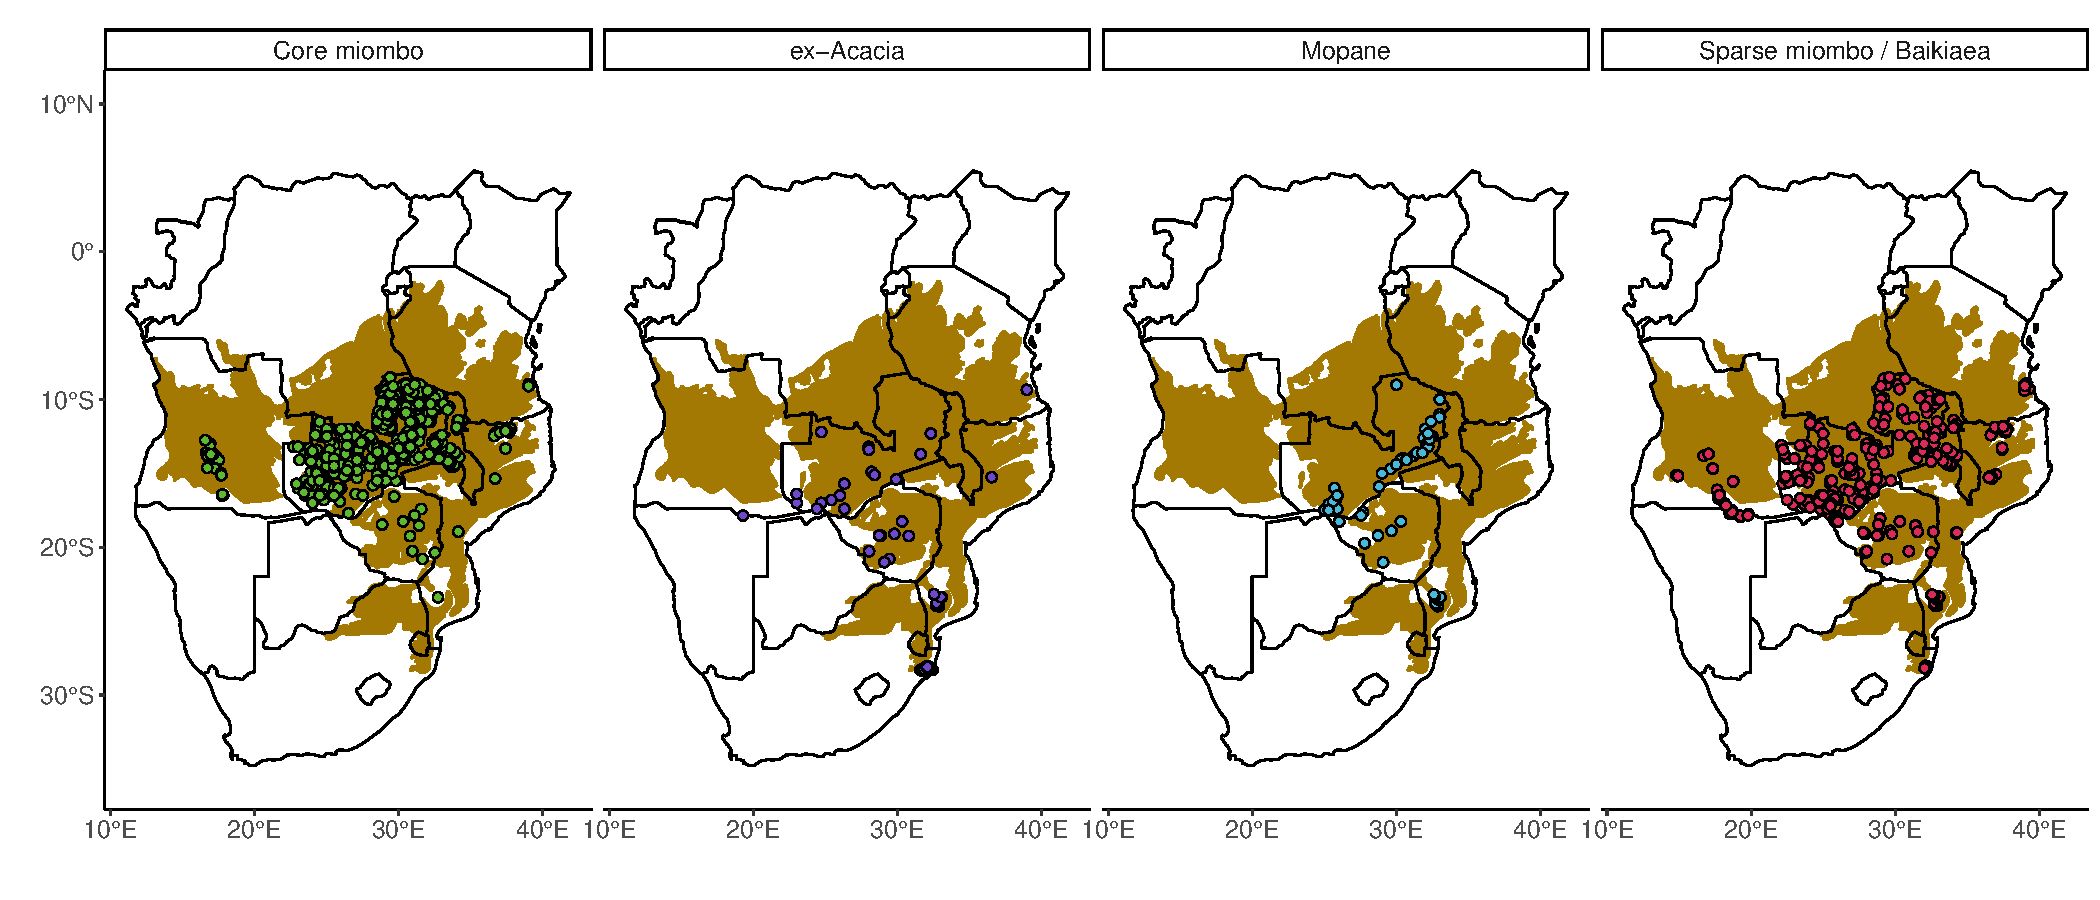
\includegraphics[width=1.4\textwidth]{clust_map}
	\caption{The locations of the \nplots{} plots used in this study, as points by geographic location with respect to the distribution of miombo woodland vegetation according to \citet{White1983}. Each panel shows plots categorized by their vegetation type as defined by the vegetation types in \autoref{clust_summ}.}
	\label{clust_map}
\end{figure}
\end{landscape}

\subsubsection*{Structural Equation Modelling}

Structural Equation Models (SEM) investigated the determinants of AGB. All SEMs were constructed and analysed in the \verb|lavaan| package \citep{lavaan} in R version 3.6.0 \citep{R2019}. SEM was used because of its suitability for modelling complex causal interactions in ecological systems \citep{Lee2007}. A key aspect to our decision to use SEMs is that they can explicitly model and partition variance to indirect effects, which is challenging in standard multiple regressions. Using SEMs also allowed us to describe theoretical latent constructs which have been suggested to act upon diversity and biomass/productivity in previous studies despite these factors not having single observable measures in our dataset. Structural equation modelling is also necessary to properly account for potential feedback mechanisms between aspects of climate and tree species diversity, which could otherwise increase the chances of Type I error and wrongly attribute inference due to covariance of explanatory variables when using conventional regression analyses \citep{Nachtigall2003}.

Prior to analysis, we specified a conceptual model with factors expected to affect AGB: moisture availability, soil fertility, tree species diversity, tree structural diversity and stem density (\autoref{con_mod}). 

\begin{figure}[H]
\centering
	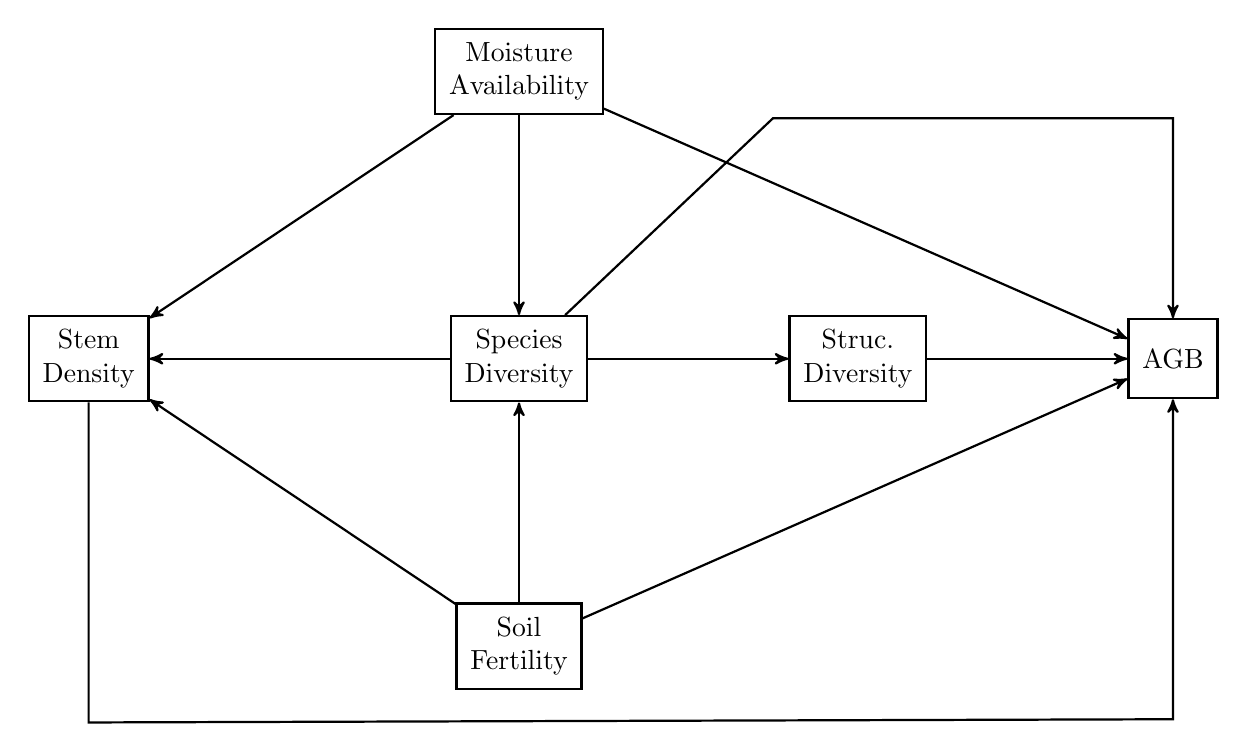
\begin{tikzpicture}[auto,scale=2, 
	observed/.style={rectangle,draw,thick,inner sep=5pt,minimum size=1cm, align=center},
	latent/.style={circle, draw, thick, inner sep=0pt, minimum size=2cm, align=center}, 
	path/.style={->, thick, >=stealth'},
	loading/.style={->, thick, dashed, >=stealth'}]

\tikzset{mystyle/.style={->,double=black}}
\node [observed] (m) {Moisture\\Availability};
\node [observed] (d) [below = 1in of m] {Species\\Diversity}; 
\node [observed] (s) [below = 1in of d] {Soil\\Fertility}; 
\node [observed] (h) [right = 1in of d] {Struc.\\Diversity}; 
\node [observed] (b) [right = 1in of h] {AGB}; 
\node [observed] (i) [left = 1.5in of d] {Stem\\Density};

\draw [path] (m) to node {} (d);
\draw [path] (s) to node[right] {} (d);
\draw [path] (d) to node[below] {} (h);
\draw [path] (h) to node {} (b);
\draw [path] (m) to node[above=0.1in, pos=0.5] {} (i);
\draw [path] (s) to node {} (i);
\draw [path] (d) to node {} (i);
\draw [path] (m) to node {} (b);
\draw [path] (s) to node[below=0.1in, pos=0.5] {} (b);

\coordinate[below= 1.6in of i] (ibleft); 
\coordinate[below= 1.6in of b] (ibright); 
\draw [path] (i) -- (ibleft) -- (ibright) -- (b);

\coordinate[above= 1in of b] (dbright);
\coordinate[left= 2in of dbright] (dbleft);
\draw [path] (d) -- (dbleft) -- (dbright) -- (b);
\end{tikzpicture}



	\caption{Conceptual Directed Acyclic Graph (DAG) showing the theoretical relationships between environmental factors, tree species diversity, tree structural diversity, tree stem density, and AGB. Hypothesised paths of causation are depicted as arrows from predictor to response. Correlations are depicted as curved dotted arrows.}
	\label{con_mod}
\end{figure}

Observed variables were transformed to achieve normality where necessary and standardised to Z-scores prior to analysis (\hyperref[appendixc]{Appendix C}). Standardisation put each latent variable on the same scale, with a mean of zero and a standard deviation of one. Standardisation allows path regression coefficients to be easily compared between paths in the same model to assess their relative effect size, and eliminates confusion in model interpretation arising from the observed variables being on different scales \citep{Beaujean2014}. Standardisation also controls for variables with different orders of magnitude which could otherwise prevent adequate model estimation from the covariance matrix in \verb|lavaan|. To ensure that observed variables within a latent variable had consistent directions of influence, some observed variables were reversed by multiplying by -1. For example, soil fertility is expected to decrease as soil sand content increases, so soil percentage sand content was reversed for model fitting. Precipitation seasonality (PS), temperature seasonality (TS), and mean annual temperature (MAT) were also reversed in this way to account for the direction of their effect on moisture availability.

%While it is recommended by some to set exact factor loadings in the SEM from the regression coefficients of multiple regressions \citep{lavaan}, because some latent variables were regressed against both structural diversity and AGB, exact factor loadings from simple multiple regressions could not be used. We therefore allowed factor loadings to be estimated by the SEM itself.

The factor loadings of the observed variable assumed to contribute most to each latent variable were set to 1 as per convention, with other observed variables being allowed to vary \citep{Beaujean2014}.  We tested the robustness of our assumptions with a chi-squared test of all possible combinations of observed variable factor loadings set to 1, while ensuring no factor loadings were in excess of 1. We found no significant difference between model specifications (p>0.05). Full Information Max-Likelihood (FIML) was used in each model to estimate the values of missing data in each latent variable \citep{Cham2017}.

We assessed the role of structural diversity and species diversity in determining AGB via a simple mediation model which allowed species diversity to influence AGB both directly and indirectly via structural diversity. To account for variation in stem density which may covary with species diversity we also included it as an predictor in our model. To explore variation in the model among woodland vegetation types, we fit the model both at the regional scale and for each vegetation cluster separately. We compared unstandardised path coefficients among these vegetation cluster scale models to understand the effect that vegetation type has on the relationship between tree species diversity, structural diversity, stem density and AGB. Path coefficients show the effect of a path with other paths of inference held constant. Models were estimated using the ``MLM'' estimator, because it is robust to multivariate non-normality \citep{Shapiro1983}. Model fit was evaluated using the robust Comparative Fit Index (CFI), the robust Tucker Lewis Index (TLI), the Root Mean Squared Error (RMSEA) and the R\textsuperscript{2} coefficient of determination for AGB. We critically assess model fit in each case, taking into consideration the recommendations of \citet{Hu1999} which define threshold values of acceptability for these model fit indices: CFI >0.85, TLI >0.85, RMSEA <0.15, alongside our judgement of the model estimates.

To explore the hypothesis that complementarity effects increase in strength as stem density increases, we repeatedly sub-sampled the available plot dataset to create \subn{} datasets of similar size with varying median stem density. We used each of these datasets separately to fit the model including only tree species and structural diversity latent variables to predict AGB. We excluded the effect of stem density on AGB and the correlation between stem density and species diversity from this model as we were deliberately controlling stem density in our subsampling. We then examined how the unstandardised path coefficients for each path in the SEM varied according to the median stem density of subsampled dataset.

We incorporated environmental covariates into our model to understand the relative effects of moisture availability and soil fertility on AGB both directly and indirectly via species diversity and stem density. We compared standardised path coefficients between paths in the model to understand the relative contribution of each path to explain variance in AGB. Vegetation type specific models could not be reliably fitted for this more complex model specification with environmental covariates, due to sample size issues and because some vegetation clusters were narrow in their climate space leading to a lack of variance particularly in moisture availability.

% We fitted separate moderation models to investigate whether there was an interaction effect whereby the strength of the relationship between species diversity and AGB was influenced by moisture availability and soil fertility. The \verb|lavaan| R package does not natively support moderation of latent variables in its model specification. Instead we manually calculated interaction variables for both soil fertility and moisture availability from the product of predicted values of these latent variables in a Confirmatory Factor Analysis (CFA). Interaction variables were the products: tree species diversity $\times$ moisture availability, and tree species diversity $\times$ soil fertility. These interaction terms were included as explanatory terms in multiple regressions alongside the latent variable of species diversity to predict AGB. Regression coefficients and model fit were analysed to determine the presence and form of interaction effects.

\section*{Results}

\begin{figure}[H]
\centering
	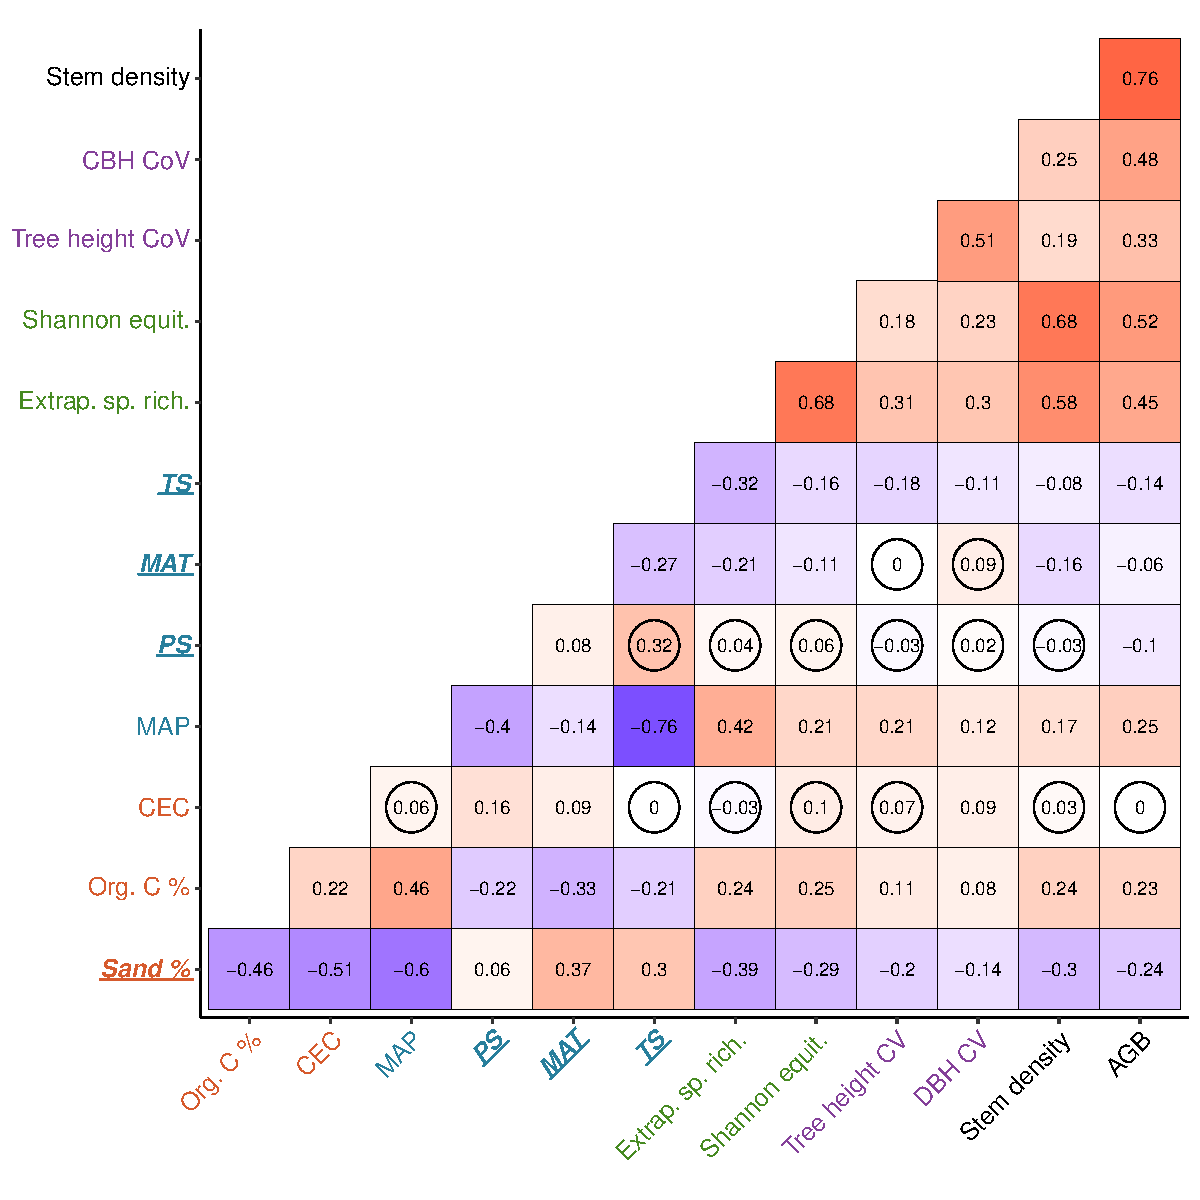
\includegraphics[width=0.6\textwidth]{corr_mat}
	\caption{Correlogram of standardised observed variables used in the SEMs, with Pearson correlation coefficients ($r$) coloured according to sign ($+$ve red, $-$ve blue) and shaded by strength of correlation. Variables in bold and underlined on the axis labels were later reversed for SEMs to maintain positive correlations for all observed variables within each latent variable. Correlation coefficients marked by a circle indicate that the 95\% confidence interval of this correlation overlapped zero. Colours of variable names group them into latent variables used in the SEMs: red = soil fertility, blue = moisture availability, green = tree species diversity, purple = tree structural diversity. See \hyperref[appendixd]{Appendix D} for a full assessment of correlation fit statistics.}
	\label{corr_mat}
\end{figure}

Pairwise correlations between all observed variables used in the Structural Equation Models (SEMs) showed that all tree species diversity and structural diversity variables had moderate positive correlations with AGB. Stem density had the strongest correlation with AGB of all variables (\ccib{}). Environmental variables had weaker correlations with AGB than diversity variables, with all environmental variables having significant correlations with AGB, except CEC and MAT.

The direction of these correlations was used as a test of our assumptions of the direction of influence of latent variables later used in the SEMs. As expected, there was a positive correlation between MAP and AGB (\ccmb{}), and a weak negative correlation between the seasonality of precipitation and AGB (\ccmcb{}). MAT and temperature seasonality (TS) negatively correlated weakly with AGB (MAT: \cctb{}; TS: \cctcb{}). As expected, there was a negative correlation between soil sand content and AGB (\ccsb{}), and a positive correlation between soil organic carbon and AGB (\ccob{}). 

MAP had positive correlations with tree species richness (\ccms{}), abundance evenness (\ccme{}), tree height diversity (\ccmh{}) and tree stem density (\ccmi{}). MAT had weak correlations with tree species and structural diversity variables. Tree species diversity variables had clear positive correlations with stem density (Species richness: \ccsi{}; Shannon equitability: \ccei{}). 

\subsection*{Structural and species diversity models}

In an SEM describing the effect of tree species diversity on AGB via the mediating effects of stand structural diversity and stem density (\autoref{struc_mod}), species diversity had a small positive direct effect on AGB (\strucdb{}), and indirectly via structural diversity (\strucdsb{}) (\autoref{struc_mod}). Tree species diversity had a positive correlation with stem density. Model fit was good with high factor loadings for all observed variables, all path coefficients were significant (p <0.01) (\autoref{struc_model_fit_clust_stats}). The R\textsuperscript{2} of AGB was \strucrsq{}. The strongest direct effect on AGB was from stem density (\strucsib{}).

\begin{figure}[H]
\centering
	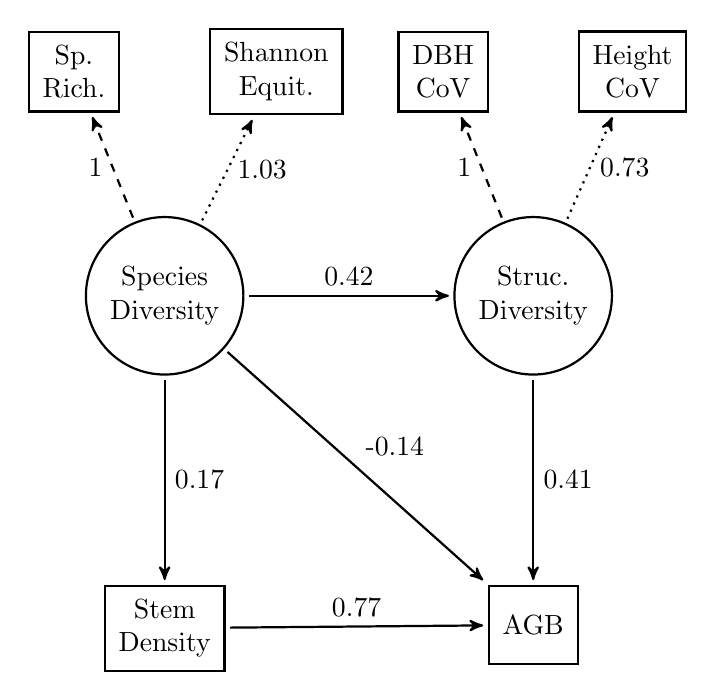
\begin{tikzpicture}[auto,scale=2, 
	observed/.style={rectangle,draw,thick,inner sep=5pt, outer sep=2pt, minimum size=1cm, align=center},
	latent/.style={circle, draw, thick, inner sep=0pt, outer sep=2pt, minimum size=2cm, align=center}, 
	path/.style={->, thick, >=stealth'},
	loading/.style={->, thick, dotted, >=stealth'},
	loadingset/.style={->, thick, dashed, >=stealth'}]

\tikzset{mystyle/.style={->,double=black}}
\node [latent] (d) {Species\\Diversity}; 
\node [latent] (h) [right = 1in of d] {Struc.\\Diversity}; 
\node [observed] (b) [below = 1in of h] {AGB}; 
\node [observed] (i) [below = 1in of d] {Stem\\Density};

\coordinate[above= 0.7in of d] (domid);
\coordinate[above= 0.7in of h] (homid);
\node [observed] (ds) [left = 0.2in of domid] {Sp.\\Rich.};
\node [observed] (de) [right = 0.2in of domid] {Shannon\\Equit.};
\node [observed] (hd) [left = 0.2in of homid] {DBH\\CoV};
\node [observed] (hh) [right = 0.2in of homid] {Height\\CoV};


\draw [loadingset] (d) to node[left, pos=0.5] {\pcsdsd{}} (ds);
\draw [loading] (d) to node[right, pos=0.5] {\pcsded{}} (de);
\draw [loadingset] (h) to node[left, pos=0.5]  {\pcshdh{}} (hd);
\draw [loading] (h) to node[right, pos=0.5] {\pcshhh{}} (hh);

\draw [path] (d) to node {\pcsdh{}} (h);
\draw [path] (h) to node {\pcshb{}} (b);
\draw [path] (d) to node {\pcsdi{}} (i);
\draw [path] (i) to node {\pcsib{}} (b);
\draw [path] (d) to node {\pcsdb{}} (b);

\end{tikzpicture}


	\caption{Path diagram with regression coefficients for the tree diversity SEM, including plots from all vegetation clusters. Latent variables are circles while observed variables are rectangles. Standardised path coefficients are solid arrows pointing from predictor to response with the effect size of the path coefficient expressed in terms of standard deviations on the latent variable response scale. The observed variables which inform the latent variables are connected by dotted arrows, observed variables with loading set to 1 are connected by dashed arrows. Correlations between variables are depicted as dotted curved arrows. Measurement errors of exogenous variables are omitted for clarity.}
	\label{struc_mod}
\end{figure}

\subsection*{Variation among vegetation types}

When the tree species and structural diversity model (\autoref{struc_mod}) was refitted separately using data from each of the 4 vegetation types the strengths of unstandardised path coefficients varied.  The direct effect of tree species diversity on AGB was positive in Baikiaea and Mopane, but negative in Marginal and Core miombo (\autoref{struc_model_slopes_all}). Relationships between structural diversity and AGB remained generally similar with the same sign and significant overlap between the 95\% confidence intervals of path coefficients. The total effect of species diversity on AGB remained strongly positive for all vegetation types. All vegetation types except Mopane exhibited a positive effect of species diversity on structural diversity. All models had adequate goodness-of-fit (\autoref{struc_model_fit_clust_stats}), though confidence intervals around the unstandardised path coefficients were wide particularly for Mopane and Baikiaea. $\chi^{2}$ statistics were high for some vegetation types, but this appears to be highly correlated with sample size for each vegetation type \citep{Hooper2008}.

The strongest total effect of tree species diversity on AGB was in Baikiaea woodland (\struccsb{}), which was species rich but highly variable in species diversity compared to other vegetation types (\autoref{clust_summ}). The R\textsuperscript{2} of AGB was highest in Marginal miombo (R\textsuperscript{2} = \strucarsq{}) and lowest in the Core miombo (R\textsuperscript{2} = \\strucbrsq{}strucbrsq{}).

\begin{figure}[H]
\centering
	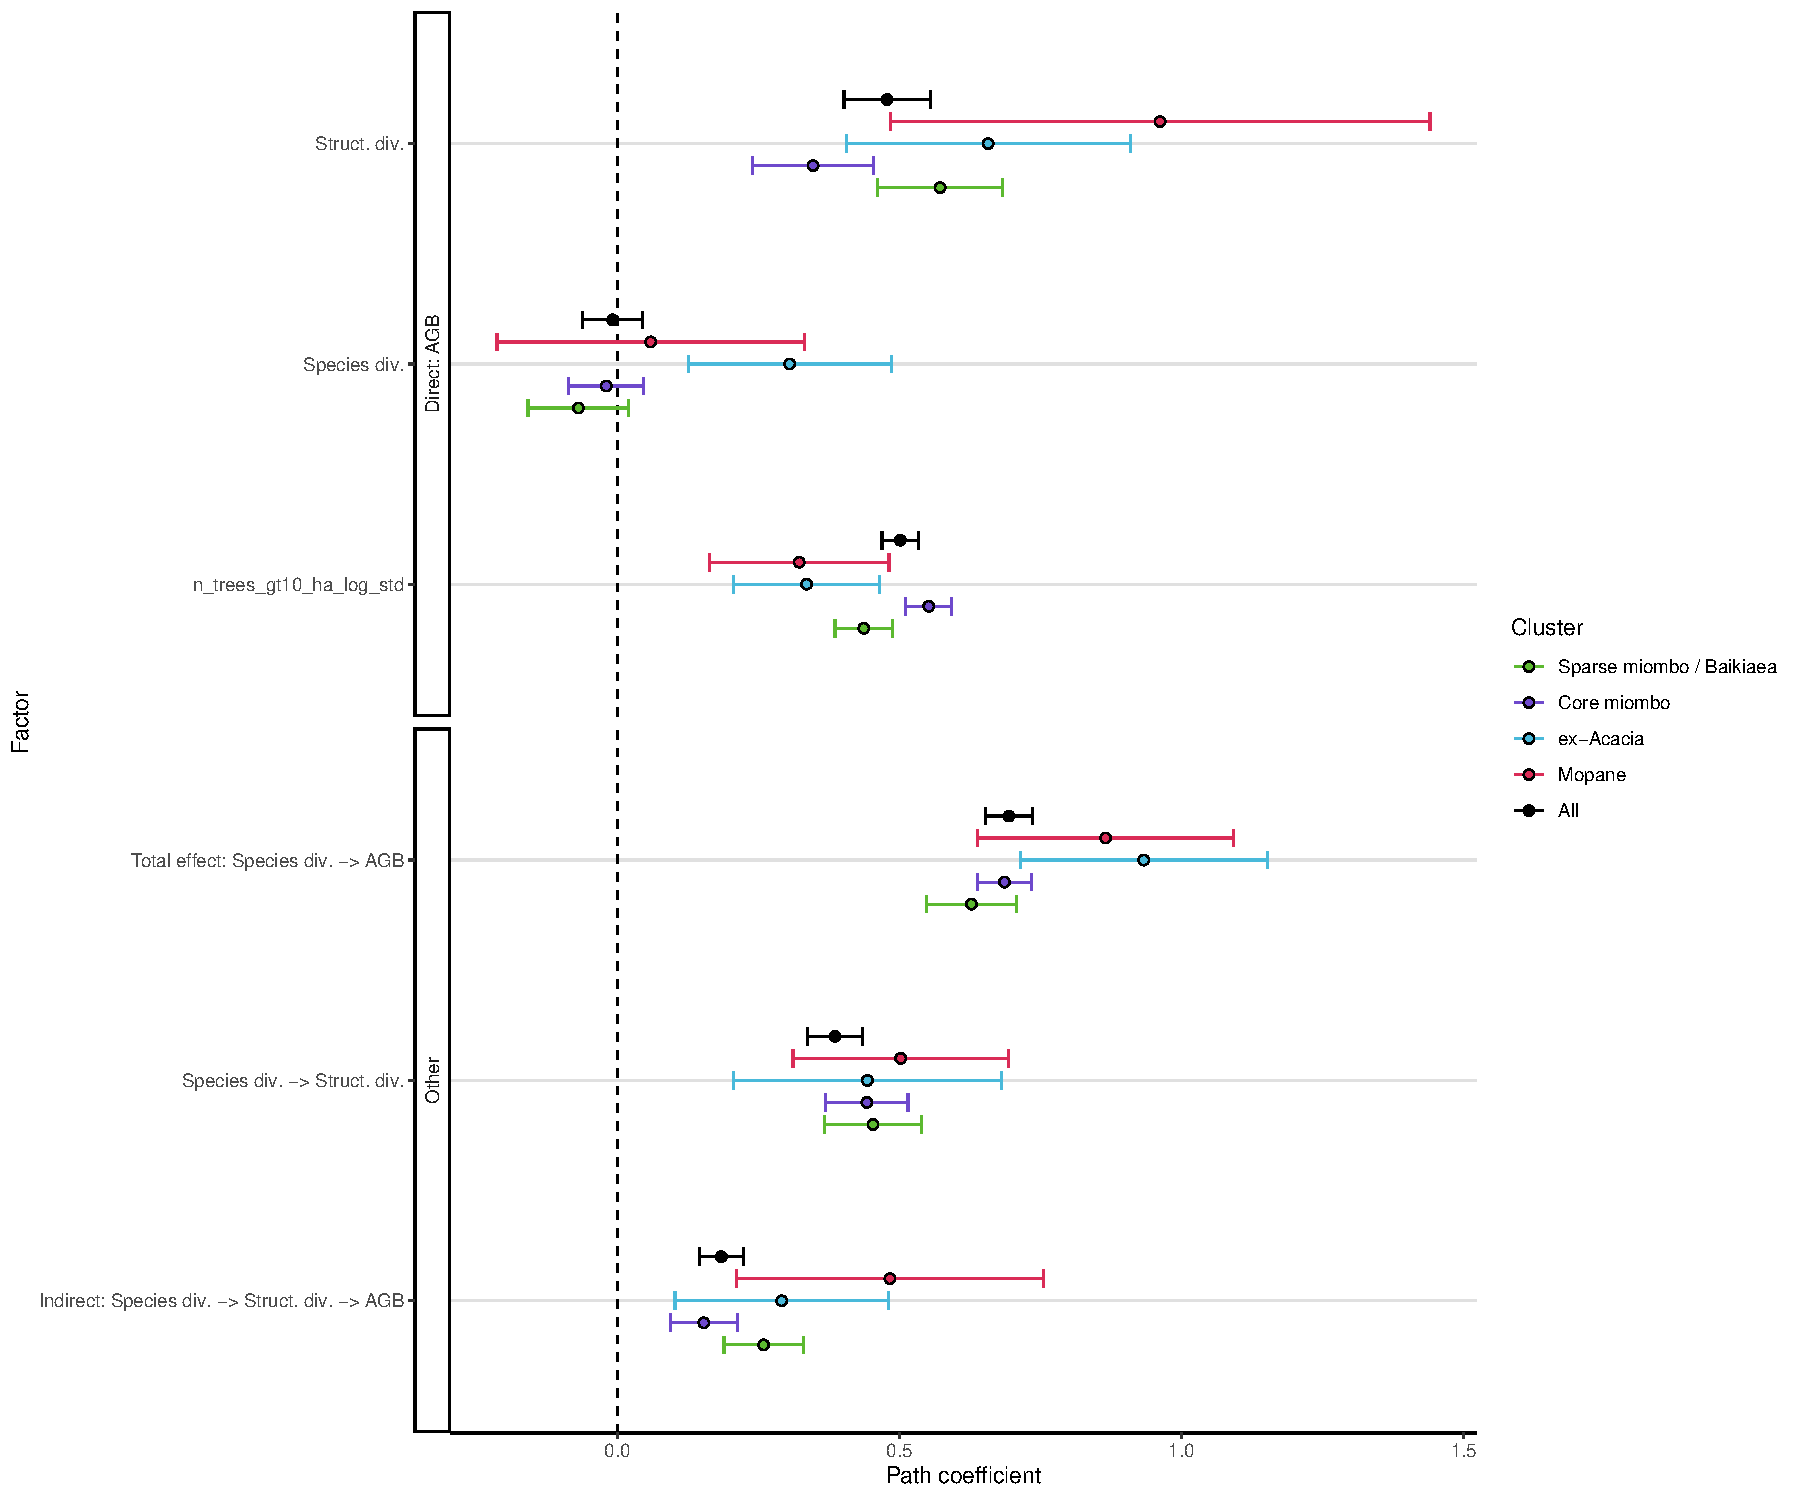
\includegraphics[width=\textwidth]{struc_model_slopes_all}
	\caption{Unstandardised path coefficients for the effects of tree diversity on AGB, mediated by the effect of stand structural diversity. Path coefficients are $\pm$1 standard error. Path coefficients where the standard error does not overlap zero are considered to be significant effects.}
	\label{struc_model_slopes_all}
\end{figure}


% Table created by stargazer v.5.2.2 by Marek Hlavac, Harvard University. E-mail: hlavac at fas.harvard.edu
% Date and time: Fri, Jan 17, 2020 - 12:26:16
\begin{table}[!htbp] \centering 
  \caption{} 
  \label{struc_model_fit_clust_stats} 
\begin{tabular}{@{\extracolsep{5pt}} ccccccccc} 
\\[-1.8ex]\hline 
\hline \\[-1.8ex] 
cluster & ntotal & chisq & df & cfi & tli & logl & rmsea & rsquare\_agb \\ 
\hline \\[-1.8ex] 
Marginal miombo & $525$ & $44.750$ & $6$ & $0.966$ & $0.916$ & $$-$3714.000$ & $0.110$ & $0.710$ \\ 
Core miombo & $668$ & $57.210$ & $6$ & $0.962$ & $0.904$ & $$-$4224.000$ & $0.100$ & $0.680$ \\ 
Baikiaea & $47$ & $5.860$ & $6$ & $0.998$ & $0.994$ & $$-$324.600$ & $0.030$ & $0.720$ \\ 
Mopane & $84$ & $9.420$ & $6$ & $0.971$ & $0.927$ & $$-$591.600$ & $0.080$ & $0.450$ \\ 
All & $1324$ & $78.430$ & $6$ & $0.975$ & $0.936$ & $$-$9119.000$ & $0.090$ & $0.690$ \\ 
\hline \\[-1.8ex] 
\end{tabular} 
\end{table} 


\subsection*{Moderation of Diversity-AGB relationship by stem density}

\rchange{We repeatedly sub-sampled the plot dataset to build \subn{} datasets of varying mean stem density in order to test how the relationship between species diversity, structural diversity and biomass varied with stem density. Each dataset consisted of approximately \subp{} plots with overlap of plot identity between subsampled datasets.  \autoref{sem_struc_stems_ha} shows a positive effect of tree species diversity on AGB as stem density increases.}{In our sub-sampling of the plot dataset by mean stem density, we found a positive effect of tree species diversity on AGB as stem density increases (\autoref{sem_struc_stems_ha})}. There appears to be a minimum stem density threshold at \textapprox{}180 stems ha\textsuperscript{-1} below which there appears to be a reasonably constant low baseline effect of tree diversity on biomass. The effect of structural diversity on AGB appears to remain constant with increasing stem density. The indirect effect of species diversity on AGB via structural diversity climbs slightly as stem density increases.

\begin{figure}[H]
\centering
	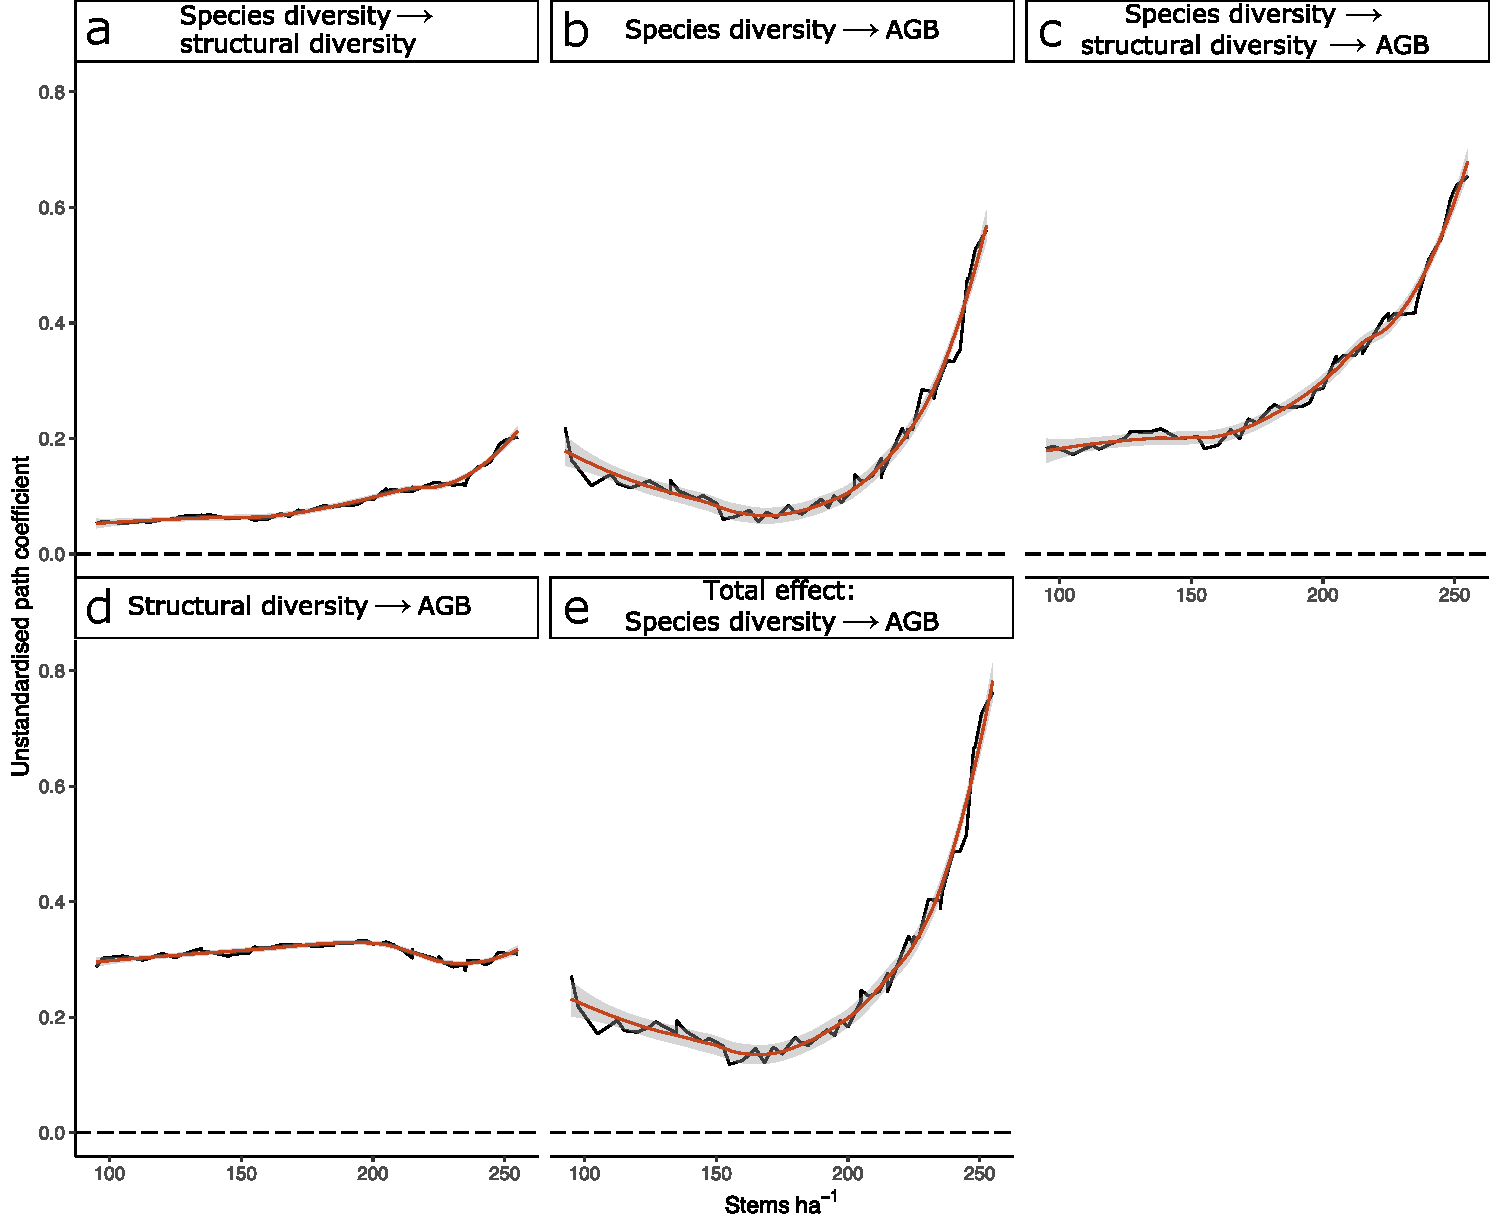
\includegraphics[width=0.8\textwidth]{sem_struc_stems_ha}
	\caption{Line plots showing the variation in path coefficients in the SEM, using datasets with different mean stem density. Smoothed lines are loess curves with standard error shaded bars.}
	\label{sem_struc_stems_ha}
\end{figure}

\subsection*{Environmental covariates and diversity}

A model incorporating the latent variables of moisture availability and soil fertility showed that the total effect of species diversity on biomass was greater than that of both moisture availability and soil fertility (\autoref{full_mod}). Surprisingly, the direct effects of moisture availability and soil fertility on biomass were negligible, with nearly all of their observed effect on AGB coming from the indirect path via species diversity (moisture: \rgmbd{}, soil: \rgsbd{}). MAP and temperature seasonality (TS) had the greatest contributions to the latent variable of moisture availability. Moisture availability and soil fertility also had negligible direct effects on stem density.  Model fit was acceptable: CFI = \fmcfi{}, TLI = \fmtli{}, and RMSEA = \fmrmsea{}, R\textsuperscript{2} of AGB = \fmrsq{}.

Similar to the model which only considered tree species and structural diversity (\autoref{struc_mod}), the direct effect of species diversity on structural diversity was positive, while structural diversity itself had a positive effect on AGB, leading to a strong positive indirect effect of species diversity on AGB via structural diversity (\rgbhd{}). The total effect of species diversity on AGB was positive (\rgbd{}).

\begin{figure}[H]
\centering
	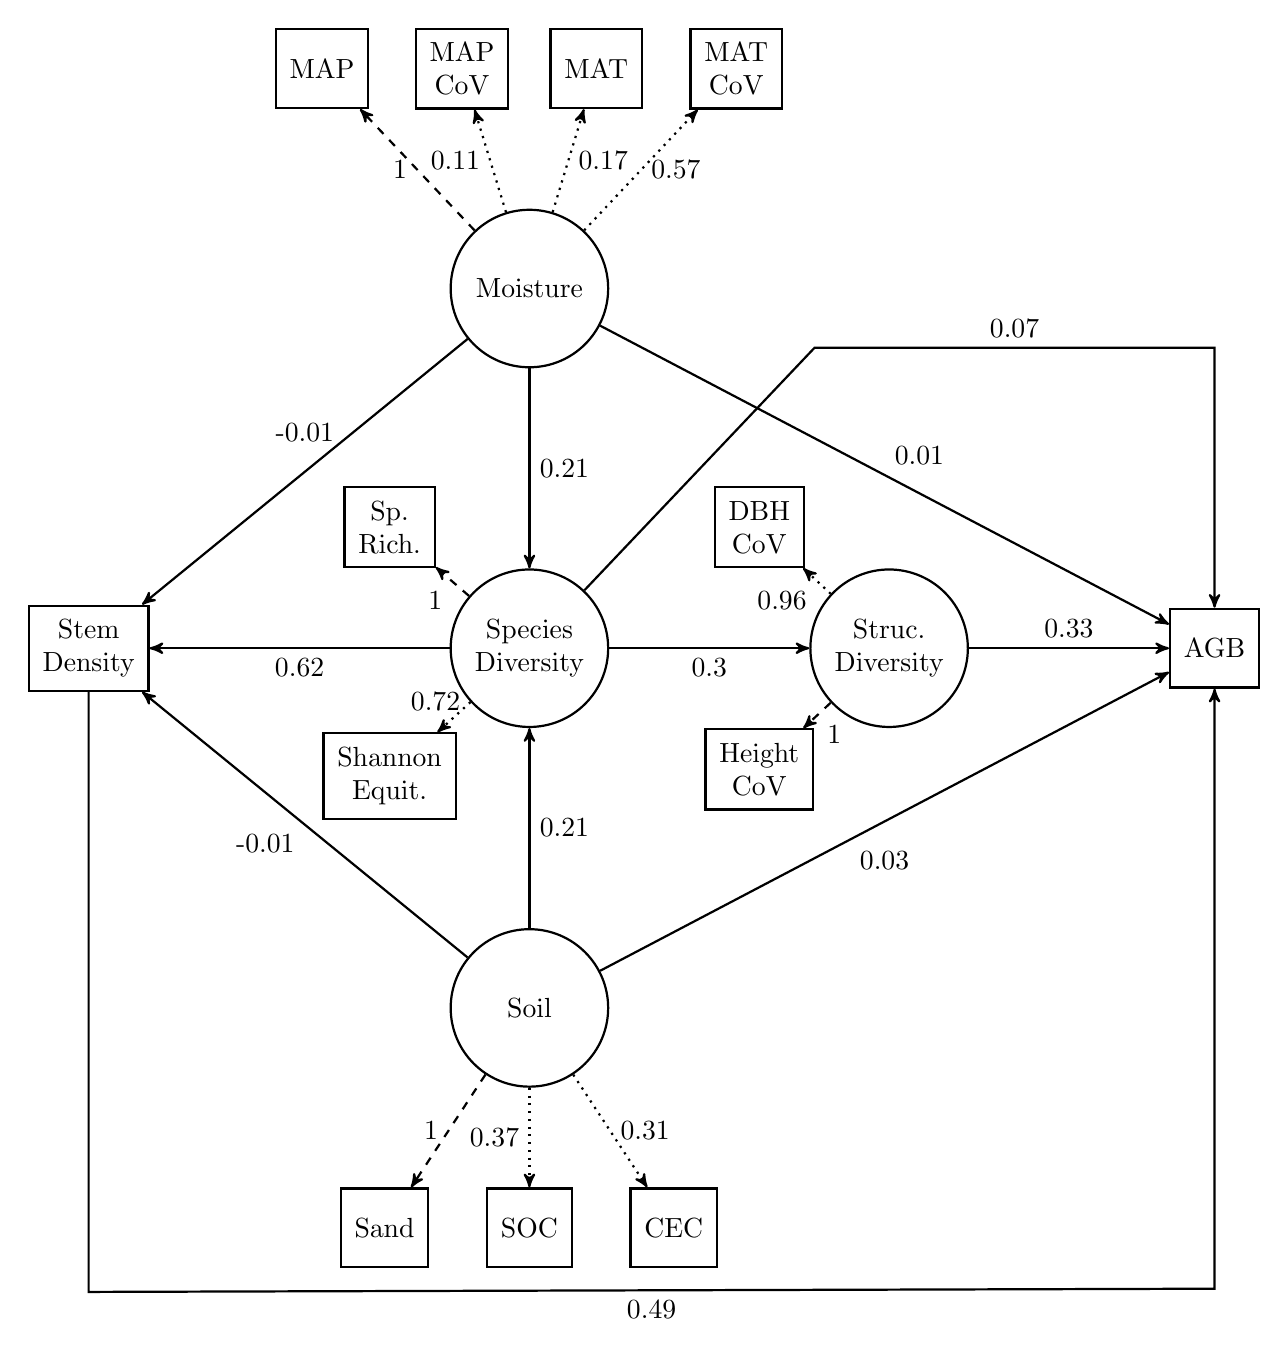
\begin{tikzpicture}[auto,scale=2, 
	observed/.style={rectangle,draw,thick,inner sep=5pt,minimum size=1cm, align=center},
	latent/.style={circle, draw, thick, inner sep=0pt, minimum size=2cm, align=center}, 
	path/.style={->, thick, >=stealth'},
	loading/.style={->, thick, dotted, >=stealth'},
	loadingset/.style={->, thick, dashed, >=stealth'}]

\tikzset{mystyle/.style={->,double=black}}
\node [latent] (m) {Moisture};
\node [latent] (d) [below = 1in of m] {Species\\Diversity}; 
\node [latent] (s) [below = 1in of d] {Soil}; 
\node [latent] (h) [right = 1in of d] {Struc.\\Diversity}; 
\node [observed] (b) [right = 1in of h] {AGB}; 
\node [observed] (i) [left = 1.5in of d] {Stem\\Density};

\coordinate[above= 0.7in of m] (momid);
\node [observed] (mp) [left = 0.8in of momid] {MAP};
\node [observed] (mpc) [left = 0.1in of momid] {MAP\\CoV};
\node [observed] (mt) [right = 0.1in of momid] {MAT};
\node [observed] (mtc) [right = 0.8in of momid] {MAT\\CoV};

\coordinate[below= 0.7in of s] (somid);
\node [observed] (ss) [left = 0.5in of somid] {Sand};
\node [observed] (sc) at (somid) {SOC};
\node [observed] (so) [right = 0.5in of somid] {CEC};

\coordinate[left= 0.3in of d] (domid);
\node [observed] (ds) [above = 0.4in of domid] {Sp.\\Rich.};
\node [observed] (de) [below = 0.42in of domid] {Shannon\\Equit.};

\coordinate[left= 0.25in of h] (homid); 
\node [observed] (hd) [above = 0.4in of homid] {DBH\\CoV};
\node [observed] (hh) [below = 0.4in of homid] {Height\\CoV};


\draw [path] (m) to node {\pcfmd{}} (d);
\draw [path] (s) to node[right] {\pcfsd{}} (d);
\draw [path] (d) to node[below] {\pcfdh{}} (h);
\draw [path] (h) to node {\pcfhb{}} (b);
\draw [path] (m) to node[above=0.1in, pos=0.5] {\pcfmi{}} (i);
\draw [path] (s) to node {\pcfsi{}} (i);
\draw [path] (d) to node {\pcfdi{}} (i);
\draw [path] (m) to node {\pcfmb{}} (b);
\draw [path] (s) to node[below=0.1in, pos=0.5] {\pcfsb{}} (b);

\draw [loadingset] (m) to node[left, pos=0.5] {\pcfmmp{}} (mp);
\draw [loading] (m) to node[left, pos=0.5] {\pcfmmpc{}} (mpc);
\draw [loading] (m) to node[right, pos=0.5] {\pcfmmt{}} (mt);
\draw [loading] (m) to node[right, pos=0.5] {\pcfmmtc{}} (mtc);

\draw [loadingset] (s) to node[left, pos=0.5] {\pcfsss{}} (ss);
\draw [loading] (s) to node[left, pos=0.5] {\pcfssc{}} (sc);
\draw [loading] (s) to node[right, pos=0.5] {\pcfsso{}} (so);

\draw [loadingset] (d) to node {\pcfdds{}} (ds);
\draw [loading] (d) to node[left, pos=0] {\pcfdde{}} (de);

\draw [loading] (h) to node[] {\pcfhhd{}} (hd);
\draw [loadingset] (h) to node {\pcfhhh{}} (hh);

\coordinate[below= 3in of i] (ibleft); 
\coordinate[below= 3in of b] (ibright); 
\draw [path] (i) -- (ibleft) to node[below] {\pcfib{}} (ibright) -- (b);

\coordinate[above= 1.3in of b] (dbright);
\coordinate[left= 2in of dbright] (dbleft);
\draw [path] (d) -- (dbleft) to node[above] {\pcfdb{}} (dbright) -- (b);

\end{tikzpicture}



	\caption{Path diagram with regression coefficients for the SEM incorporating environmental covariates and tree species and structural diversity across all five vegetation types. Latent variables are shown as circles while observed variables are shown as rectangles. Standardised path coefficients are solid arrows pointing from predictor to response with the effect size of the path coefficient expressed in terms of standard deviations on the latent variable response scale. Observed variables which inform the latent variables are connected by dotted arrows, observed variables with loading set to 1 are connected by dashed arrows. Correlations between variables are depicted as dotted curved arrows. Measurement errors of exogenous variables are omitted for clarity.}
	\label{full_mod}
\end{figure}

% 
% Table created by stargazer v.5.2.2 by Marek Hlavac, Harvard University. E-mail: hlavac at fas.harvard.edu
% Date and time: Tue, Oct 29, 2019 - 10:25:05
\begin{table}[!htbp] \centering 
  \caption{} 
  \label{full_model_fit_clust_stats} 
\begin{tabular}{@{\extracolsep{5pt}} ccccccccccc} 
\\[-1.8ex]\hline 
\hline \\[-1.8ex] 
cluster & npar & ntotal & chisq & df & cfi & tli & logl & aic & rmsea & srmr \\ 
\hline \\[-1.8ex] 
C1 & $25$ & $420$ & $1259.430$ & $53$ & $0.460$ & $0.327$ & $$-$6145.100$ & $12340.200$ & $0.230$ & $0.187$ \\ 
C2 & $25$ & $671$ & $1530.040$ & $53$ & $0.445$ & $0.309$ & $$-$8588.900$ & $17227.900$ & $0.200$ & $0.149$ \\ 
C3 & $25$ & $105$ & $516.500$ & $53$ & $0.417$ & $0.274$ & $$-$1055.300$ & $2160.700$ & $0.290$ & $0.216$ \\ 
C4 & $25$ & $46$ & $227.910$ & $53$ & $0.457$ & $0.324$ & $$-$607.600$ & $1265.200$ & $0.270$ & $0.233$ \\ 
C5 & $25$ & $84$ & $489.700$ & $53$ & $0.387$ & $0.237$ & $$-$1097.700$ & $2245.400$ & $0.310$ & $0.328$ \\ 
\hline \\[-1.8ex] 
\end{tabular} 
\end{table} 
 - Excluded, low fit

% \subsection*{Moderation effects of moisture availability and soil}
% 
% To address the hypothesis (H\textsubscript{1}) that more arid plots and plots with less fertile soil will show a stronger positive effect of tree species richness on above ground woody biomass, we fit separate linear multiple regressions with the latent variables of moisture availability and soil fertility as moderators on the relationship between species diversity and AGB.
% 
% Both soil fertility and moisture availability had small positive interaction effects on the strength of the relationship between tree species diversity and biomass (\autoref{int_plots}). The regression coefficient for the interaction effect of tree species diversity and moisture availability was significant (\moderp{}), while the interaction term of tree species diversity and soil fertility was marginally significant (\moders{}). As moisture availability increased, the effect of tree species diversity on AGB became stronger. See \autoref{mois_div_int_mod} and \autoref{soil_div_int_mod} for full regression tables.
% 
% 
% \begin{figure}[H]
% \centering
% 	\subfloat[]{
% 	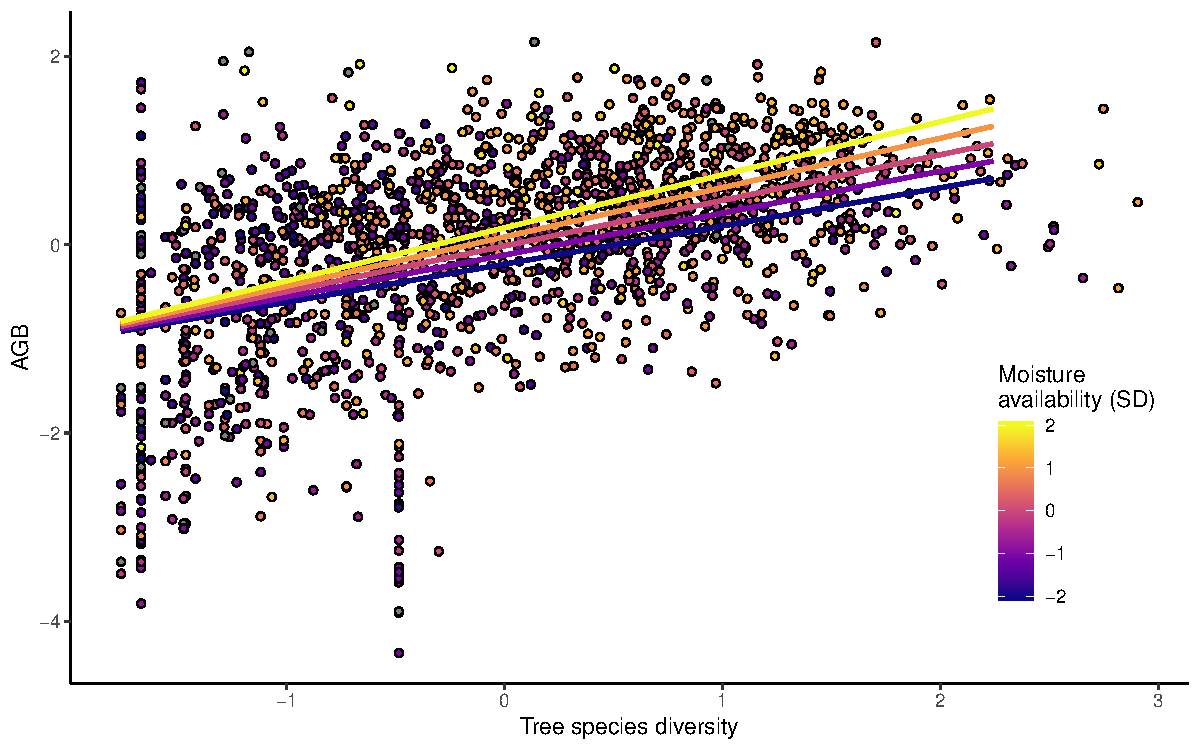
\includegraphics[width=0.48\textwidth]{mois_int}
% 	}
% 	\subfloat[]{
% 	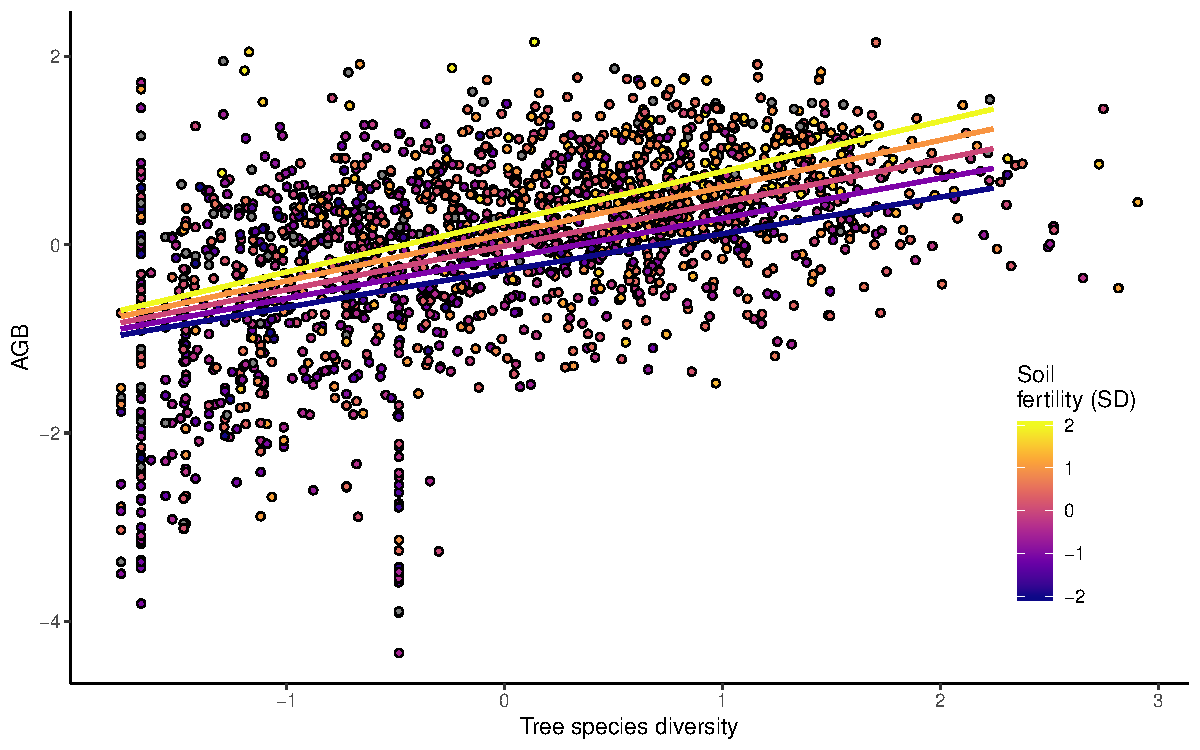
\includegraphics[width=0.48\textwidth]{soil_int}
% 	}
% 	\caption{Scatter plots showing variation in the relationship between tree species diversity and AGB with moisture availability (a) and soil fertility (b). All variables are standardised and centred to a mean of zero and a standard deviation of 1. Lines of best fit are drawn for standard deviations of moisture availability and soil fertility between -2 and +2. Moisture availability, tree species diversity and soil fertility are latent variables comprised of the same observed variable loadings.}
% 	\label{int_plots}
% \end{figure}

\section*{Discussion}

% Precipitation and soil fertility will indirectly positively effect AGB via an increase in tree species diversity.
% Tree structural diversity will indirectly influence tree species diversity to provide an indirect path of influence between structural diversity and AGB.
% The effect size of species diversity on AGB will increase with stem density, due to an increased importance of niche complementarity as competition increases.

In this study, we assessed the importance of [a] tree species richness, [b] tree structural diversity, [c] resource availability, i.e. moisture availability and soil fertility, [d] stem density and their interactions on above ground woody biomass (AGB) across SAWs, using a network of \nplots{} woodland survey plots. Using latent variables and Structural Equation Modelling (SEM), we found support for a general positive relationship between tree species diversity and AGB, with an indirect influence of tree species diversity on AGB via structural diversity (H\textsubscript{1}). We found that the effect size of tree species diversity on AGB increased with stem density (H\textsubscript{2}).  Tree diversity, structural diversity and stem density accounted for \srsq{}\% of the variation in AGB across the region, while models for specific vegetation types showed even greater explanatory power in some cases (\autoref{struc_model_fit_clust_stats}). The strongest effect on AGB was that of stem density. Interestingly, when the effects of tree species diversity, structural diversity and stem density were controlled for, we found little evidence of a direct effect of resource availability, in the form of moisture or soil fertility, on AGB (H\textsubscript{3}). 

\subsection*{Inter-related effects of tree species and structural diversity on AGB}

We found a consistent positive effect of tree species diversity on AGB across all models in this study. Within SAWs we therefore find support that higher tree species richness and evenness causes higher woody AGB. This finding is in agreement with many other studies across different ecosystems and biomes, supporting that there is a generalisable positive association between diversity and ecosystem function \citep{Liang2016, Cardinale2009}. Our study provides a novel dissection of the mechanisms underlying this relationship, particularly in the context of SAWs, a disturbance-structured and poorly studied ecological system.

% In our extrapolation of species richness according to sampling effort (stem density) we partially accounted for this effect, but our analyses cannot properly assess to what extent a real effect of species diversity on stem density exists. We cannot decompose the relative effects of tree species richness and abundance evenness in our model, but previous studies have shown that both richness and evenness have similar importance in their effects on ecosystem function \citep{Valery2009, Zhang2012}.

Much of the total variation in AGB was driven by variation in stem density. Stem density also correlated with species diversity in our SEMs. It is possible that within SAWs a higher species diversity allows for a greater density of tree stems, leading to an increase in total AGB. The opposite is also plausible however, with increased stem density causing higher species richness through an increased probability of encountering new species. We suggest that an increase in tree species diversity through species richness and evenness produces an assemblage of species which can occupy a greater proportion of the total woodland canopy volume with leaf area, utilising more of the available light resulting in greater total AGB at the plot level \citep{}. This is supported by the moderately strong indirect positive effect of tree species diversity on AGB via structural diversity.

% KGD: There are counter-examples, e.g. Johnson et al. 2016. GCB (from Leeds group, Tim Baker senior author), but feel free to leave text as is for now.

% The question of whether lots of small stems or a few large stems maximises AGB has yet to be solved \citep{}.

% While we did not explicitly measure Net Primary Productivity (NPP) in this study, other studies have shown a strong positive correlation between woody AGB and NPP in woodland and forest ecosystems \citep{Chisholm2013, Prado-Junior2016}. This suggests that, as has been found in many other woodland/forest ecosystems, woody biomass and woody productivity in SAWs can be maximised by increasing species diversity. 

We found evidence that tree species diversity led to an increase in AGB indirectly via tree structural diversity and we therefore find support for our hypothesis (H\textsubscript{2}). A higher tree species diversity allows for a greater structural diversity of trees, i.e. greater variation in DBH and height. This may act as a mechanism of niche complementarity, with a highly diverse canopy being able to take advantage of a greater proportion of the available light. Although we did not measure it here, we would also expect that tree species diversity allows for a greater range of tree functional forms \citep{}, i.e. wider variation in canopy shape and overall growth form; bushy understorey vs. emergent canopy, for example. Variation in structural diversity may be a joint result of disturbance history and tree species diversity, with highly disturbed plots generally having a less structurally diverse canopy \citep{LaRue2019}. In forests, where the tree canopy is effectively closed, as the stand matures a more diverse canopy emerges via competition and tree mortality events which open canopy gaps \citep{Muscolo2014}. Indeed, our finding that the strength of the effect of tree diversity on AGB increases with stem density supports this. In frequently disturbed woodlands such as those studied here however, a woodland canopy similar to that of a forest is frequently not reached, Instead, a simple open canopy is maintained that can be made more complex and productive via an increase in species diversity. While we did not have access to adequate data on disturbance history in our plots, previous studies have found that SAWs with higher species diversity tend to be less disturbed and tend to form a more closed canopy \citep{Chidumayo2013, Mutowo2012}.

We found a non linear positive effect of stem density on the relationship between tree species diversity and AGB (\autoref{sem_struc_stems_ha}). At low stem densities competition between trees may not occur, meaning that the niche complementarity provided by an increase in tree species richness might not make any difference to plot level AGB, accounting for the low and constant effect of tree species diversity on AGB below \textapprox{}180 stems ha\textsuperscript{-1}.

\subsection*{Effects of moisture availability and soil fertility}

Surprisingly, moisture availability and soil fertility had only small effects on AGB compared to that of tree species diversity. We expected that higher moisture availability and soil fertility would lead to higher AGB under the assumption that higher resource availability would allow for a greater stem density per unit area, greater productivity per unit area and additionally greater tree species diversity due to niche partitioning \citep{Kraaij2006, Shirima2015}.

Previous studies in tropical forests have shown that moisture availability increases AGB both directly and indirectly via increasing tree species diversity and via increasing stand structural diversity \citep{Ali2019a, Ali2019b, Poorter2017}. In this study, while we observed weak indirect effects via species diversity, we saw no evidence for a direct effect of moisture availability on AGB. Compared to moist tropical forests, moisture availability is more of a limiting factor to tree growth in SAWs, which are frequently droughted. It is possible that the range of observed moisture availability in this study (\textapprox{}460-1700 mm y\textsuperscript{-1}) may not have been able to capture variation in AGB. Due to the high levels of adaptation of tree species to drought conditions in southern Africa, at the large scale we conducted our experiment turnover in species composition along the moisture gradient may have obscured a direct relationship being observed between moisture availability and AGB.

In SAWs moisture availability is closely linked with the intensity of disturbance from seasonal fires. The growth of C4 grasses in wetter woodlands leads to more intense seasonal fires which limit tree growth \citep{Charles-Dominique2018}, and may also limit species diversity \citep{Linder2014}. It is possible therefore that the effect of moisture availability, which is expected to increase AGB, is confounded in its effect on AGB with the unmeasured variable of fire regime intensity, which is expected to decrease AGB. The direct effect of moisture availability on stem density may also be confounded in this way. This may also have caused us to not observe a stronger effect between moisture availability and AGB.

We expected a positive effect of soil fertility on AGB, but found no evidence of this in our models. We measured soil fertility using the observed variables of soil organic carbon content, sand particle content and Cation Exchange Capacity (CEC). In wet tropical forests a clear relationship has been observed between these variables and AGB \citep{Slik2010, MORE}. 
% KGD: You have written little about soil fertility in this section, but I think you need to. There is at least one paper which could be taken to suggest a positive relationship between AGB and soil fertility (Coelho de Souza et al. 2019. NEE, see my publications).

% In a separate set of linear multiple regressions, we found a weak positive interaction effect of moisture availability on the relationship between tree species diversity and AGB. As moisture availability increased, the relationship between tree species diversity and AGB became stronger. This is in contrast to \citet{Ratcliffe2017} who found that in European forests, a decrease in water availability due to drought led to a stronger effect of tree species diversity on AGB. They attributed this to an increase in selection effects which allowed dominance of stress tolerant species which were more likely to occur in high diversity assemblages. 

\subsection*{Vegetation type specific responses}

% KGD: See thoughts above for C3 results. C2 should be discussed even if we cannot give a good reason. It is very intriguing. The results for C4 also surprise me, as I would have expected mopane to be too species poor to be able to show a result. You can discuss how many mopane stands are monospecific and even thought such things as 'cathedral mopane' exist, where biomass can be quite high, it seems that adding even a few species to mopane can increase its total AGB (of the stands). That is cool and shows robustness of results. Basically, the fact that C3 and C4 show significant results means that your results are robust across a range of species richnesses (not just do to patterns at low, 1-6, or high, 6-12, species richness). I still have a great sense of what C1 is, so with withhold commentary on that for the moment. If it is 'disturbed miombo', then maybe something can be said about the contrast between results for C1 and C2 and the role that disturbance may play.

Core miombo and marginal miombo woodland vegetation exhibited a small negative direct effect of tree species diversity on AGB, while the total effect, incorporating the indirect effect via  structural diversity, remained positive in these vegetation types. Compared to Baikiaea and Mopane woodlands, miombo woodlands have higher median tree species richness. Baikiaea and Mopane woodlands are also dominated by fewer tree species, notably \textit{Baikiaea plurijuga} in Baikiaea woodlands and \textit{Colophospermum mopane} in Mopane woodlands which often produce large canopy dominating trees. We postulate that this negative effect of tree species richness on AGB in miombo woodlands may be due to an increase in interspecific competition through canopy crowding, but that this effect is not present in Baikiaea and Mopane woodlands, where the woodland canopy is dominated often by a single species. Higher functional redundancy among tree species in miombo woodlands may lead to smaller trees with lower AGB in the most diverse plots, more resembling thicket vegetation. Again, these highly diverse plots in miombo woodlands may be the result of disturbance which can promote a mosaic of woodland of different successional stages and stem densities. Alternatively, this small negative direct effect may be an artefact of particularly noisy data, especially given that the overall effect of diversity on AGB is positive.

Despite Mopane woodland having very low species diversity generally, with often monospecific stands \citep{Timberlake2010}, a positive effect of tree species diversity on AGB was observed. In previous studies across ecosystem types it has been found often that the effect on ecosystem function of adding species is stronger in low diversity assemblages \citep{Hector2007}. This has been attributed to an increase in functional redundancy as species diversity increases. \textit{I.e.} with more species, it is more likely that the addition of a new species will occupy the same ecological niche space as an existing species, meaning niche complementarity will not occur and competition will lead to niche partitioning, while making little difference to overall ecosystem functioning. Mopane woodlands also have a negligible effect of species diversity on structural diversity. This may be due to the species which tend to co-exist with \textit{C. mopane}, many of which are small shrub-like trees which do not grow into large canopy trees \citep{Timberlake2010}. Larger canopy trees tend to have greater variation in physical structure \citep{Seidel2019}.

Baikiaea woodland had the strongest total effect of species diversity on AGB. Baikiaea also has relatively low median species richness compared to miombo, but the addition of new species appears to make a larger difference to the AGB of these plots than in mopane woodlands. We suggest that this is due mostly to the particular identity of species found in Baikiaea woodlands and their contribution to ecosystem functioning. Unlike mopane woodlands, Baikiaea woodlands do sometimes contain species other than \textit{B. plurijuga} which grow to be high biomass canopy trees. 

\subsection*{Conclusion}

In this study we found that across southern African woodlands (SAWs), there is a generalisable positive association between tree species diversity and woody biomass as a measure of ecosystem function. Additionally, we found that much of this effect of species diversity on biomass exists as an indirect effect by increasing the structural diversity of woodland tree canopies. We found that the multiple vegetation types which comprise SAWs exhibit variation in the strength of the relationship between species diversity and woody biomass, inferring that models of regional and global biodiversity-ecosystem function relationships could benefit from including vegetation type terms and the structural properties of those vegetation types, such as structural diversity and stem density. In contrast to previous studies, we found that across the region, the direct effects of moisture availability and soil fertility on woody biomass were negligible, with most of their effect being indirectly through species and structural diversity. A gap in available data means that we could not incorporate disturbance history into our models adequately, but this factor likely plays a large part in the association between species diversity and woody biomass in SAWs.

SAWs are relied heavily upon for their ecosystem service provision, which is itself affect by ecosystem function. Resource extraction by humans in southern Africa is directly influencing biodiversity via selective tree-felling for timber, among other forest products. Our study shows that biodiversity change through human actions will have the greatest negative impact on ecosystem function in areas of high stem density and Baikiaea woodlands, which are predominantly targeted for tree felling. This raises concerns about the robustness of these ecosystems to further resource extraction and biodiversity loss.

% KGD: these conclusions are a bit dry and repetitive on earlier text. What do our results mean for woodland management? for conservation? for our understanding of basic ecological theory? As an aside, we have circled back around to niche complementarity in this discussion, but not really to selection effects or facilitation.
% Southern African woodlands are relied upon heavily for their ecosystem service provision, which is itself affected by ecosystem functionality \citep{Schulze1994}. This has raised interest in how biodiversity influences ecosystem function in these ecosystems. Resource extraction by humans directly influences biodiversity via selective tree-felling for timber, charcoal making, non-timber forest products and through land use change to agriculture \citep{Aleman2016, Ryan2016}. Climate change is also indirectly affecting the biodiversity of southern African woodlands, altering temperature and precipitation, and affecting climate seasonality which heavily influences the degree of seasonal drought and thus woodland structure \citep{Scholes2004, Eldridge2012}. While rapid biodiversity change is being observed in southern African woodlands \citep{Syampungani2009}, research into the relationship between biodiversity and ecosystem functionality remains scarce.

\bibliography{lib.bib}

\newpage{}
\appendix{}

\section*{Data accessibility statement}

\section*{Tables}

\section*{Figure legends and embedded figures}

\section*{Appendix 1 - Data cleaning process} \label{appendixa}

\begin{figure}[H]
\centering
	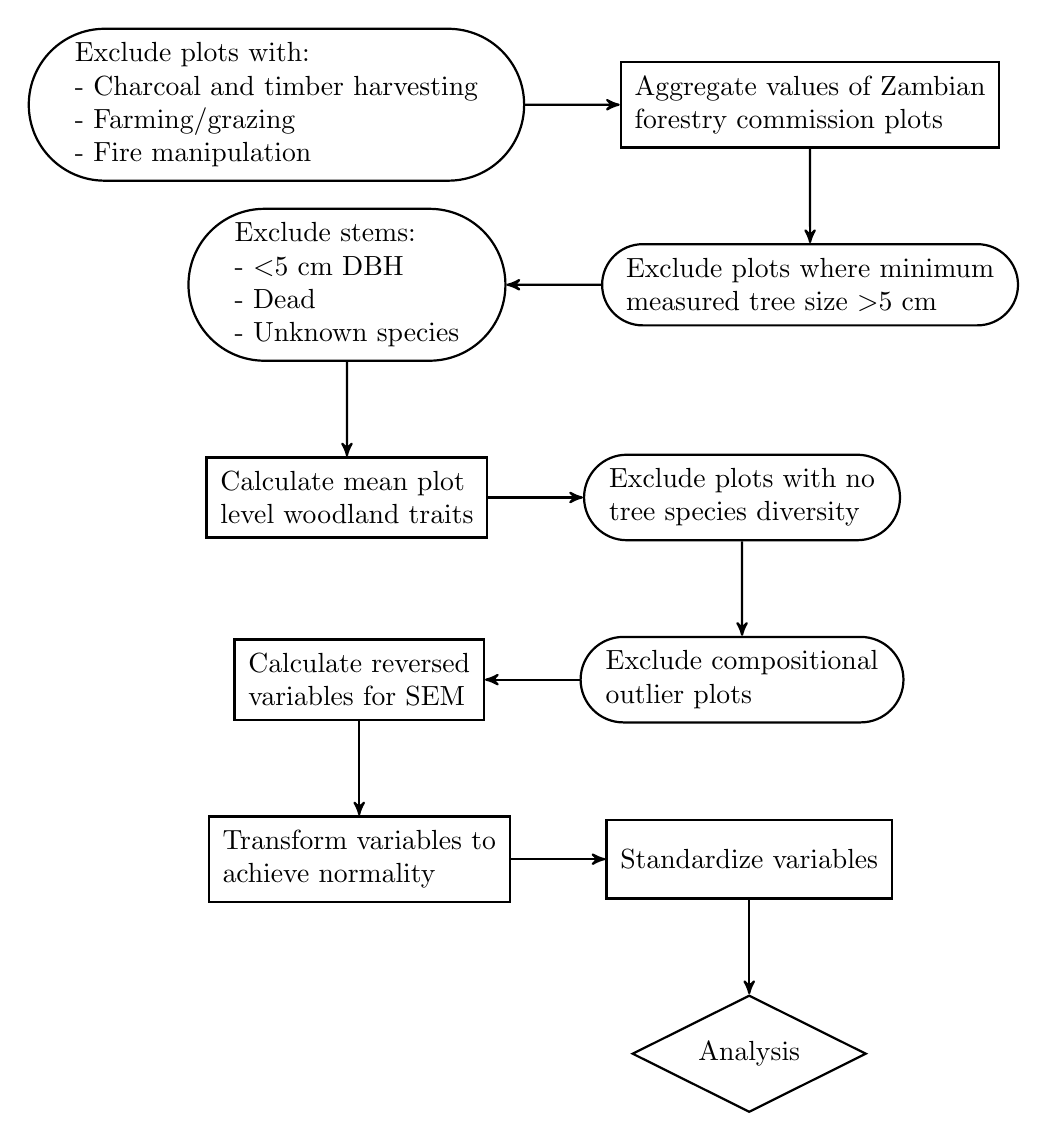
\begin{tikzpicture}[auto,scale=2, 
	round/.style={rounded rectangle,draw,thick,inner sep=5pt,minimum size=1cm, align=left},
	box/.style={rectangle,draw,thick,inner sep=5pt,minimum size=1cm, align=left},
	diam/.style={diamond,draw,thick,inner sep=5pt,minimum size=1cm, align=left, aspect=2},
	path/.style={->, thick, >=stealth'}]

\tikzset{mystyle/.style={->,double=black}}
\node  [round] (a)                    {Exclude plots with:\\- Charcoal and timber  harvesting\\- Farming/grazing\\- Fire manipulation};
\node  [box] (b) [right = 1.2cm of a] {Aggregate values of Zambian\\forestry commission plots};
\node  [round] (c) [below = 1.2cm of b] {Exclude plots where minimum\\measured tree size \textgreater{}5 cm};
\node  [round] (d) [left = 1.2cm of c] {Exclude stems:\\- \textless{}5 cm DBH\\- Dead\\- Unknown species};
\node  [box] (e) [below = 1.2cm of d] {Calculate mean plot\\level woodland traits};
\node  [round] (f) [right = 1.2cm of e] {Exclude plots with no\\tree species diversity};
\node  [round] (g) [below = 1.2cm of f] {Exclude compositional\\outlier plots};
\node  [box] (h) [left = 1.2cm of g] {Calculate reversed\\variables for SEM};
\node  [box] (i) [below = 1.2cm of h] {Transform variables to\\achieve normality};
\node  [box] (j) [right = 1.2cm of i] {Standardize variables};
\node  [diam] (k) [below = 1.2cm of j] {Analysis};
\draw [path] (a) -> (b);
\draw [path] (b) -> (c);
\draw [path] (c) -> (d);
\draw [path] (d) -> (e);
\draw [path] (e) -> (f);
\draw [path] (f) -> (g);
\draw [path] (g) -> (h);
\draw [path] (h) -> (i);
\draw [path] (i) -> (j);
\draw [path] (j) -> (k);

\end{tikzpicture}

	\caption{Flow diagram of the data filtering and cleaning process prior to analysis. Rounded boxes indicate filtering events while regular boxes indicate calculation events.}
	\label{data_clean_flow}
\end{figure}

\section*{Appendix 2 - Estimation of DBH via tree taper} \label{appendixb}

\begin{lstlisting}[language=R]
##' @title Stem diameter Point Of Measurement (POM) adjustment
##' @description  Function to estimate stem diameter at 1.3 given measurements 
##'   at other POMs.
##' @author Casey M. Ryan
##' @return d130, the estimated diameter at a POM of 1.3 m (in cm). 
##' @param d_in the diameter measured at the POM (in cm)
##' @param POM the height of the POM (in m)
##' @details The adjustment is based on a tree taper model developed as part of 
##'   the ACES project (Abrupt Changes in Ecosystem Services 
##'   https://miomboaces.wordpress.com/), using data from the miombo of Niassa. 
##'   The model is a cubic polynomial, with three equations for different sized 
##'   stems. 
##' @section Warning: The model should not be used for POMs above 1.7 m. 
##'   Extrapolating beyond the training data will give nonsense. 
##'   Thus, POMs >1.7 m are not adjusted.
##' @examples
##' POMadj(10, 0.3)
##' POMadj(1, 0.3)  # d130 is negative, i.e. the stem probably wasn't 1.3 m tall
##' POMadj(50, 1.9)  # generates warning, as outside calibration data range
##' \dontrun{
##'   POMadj(50, 0)  # zero or -ve POM is outside range, or nonsense
##' }
POMadj <- function(d_in, POM) {
  stopifnot(is.numeric(d_in),
    is.numeric(POM),
    POM >= 0,
    sum(is.na(POM))==0,
    length(POM) == length(d_in))
  if (any(POM > 1.7))
    warning("POMs >1.7 m are outside the calibration data, no correction applied")
  
  NAS <- is.na(d_in)
  d_in_clean <- d_in[!NAS]
  POM_clean <- POM[!NAS]
  # define the size class edges:
  edges <- c(5.0, 15.8, 26.6, 37.4)
  sm <- d_in_clean < edges[2]
  med <- d_in_clean >= edges[2] & d_in_clean < edges[3]
  lg <- d_in_clean >= edges[3]
  
  # compute apredictions for delta_d, for all size classes
  delta_d <- data.frame(
    # if small:
    small =  3.4678+-5.2428 * 
   	  POM_clean + 2.9401 * 
      POM_clean^2+-0.7141 * 
      POM_clean^3,
    # if med
    med =  4.918+-8.819 * 
      POM_clean + 6.367 * 
      POM_clean^2+-1.871 * 
      POM_clean^3,
    # if large
    large =  9.474+-18.257 * 
      POM_clean + 12.873 * 
      POM_clean^2+-3.325 * 
      POM_clean^3
  )
  # index into the right size class
  dd <- NA_real_
  dd[sm] <- delta_d$small[sm]
  dd[med] <- delta_d$med[med]
  dd[lg] <- delta_d$large[lg]
  dd[POM_clean > 1.7] <- 0  # to avoid extrapolation mess
  
  # add NAs back in
  d130 <- NA
  d130[NAS] <- NA
  d130[!NAS] <- d_in_clean - dd
  
  if (any(d130[!NAS] < 0))
    warning("Negative d130 estimated, repaced with NA")
  d130[d130 <= 0 & !is.na(d130)] <- NA
  return(d130)
}
\end{lstlisting}

\section*{Appendix 3 - Frequency distribution of observed variables} \label{appendixc}

\begin{figure}[H]
\centering
	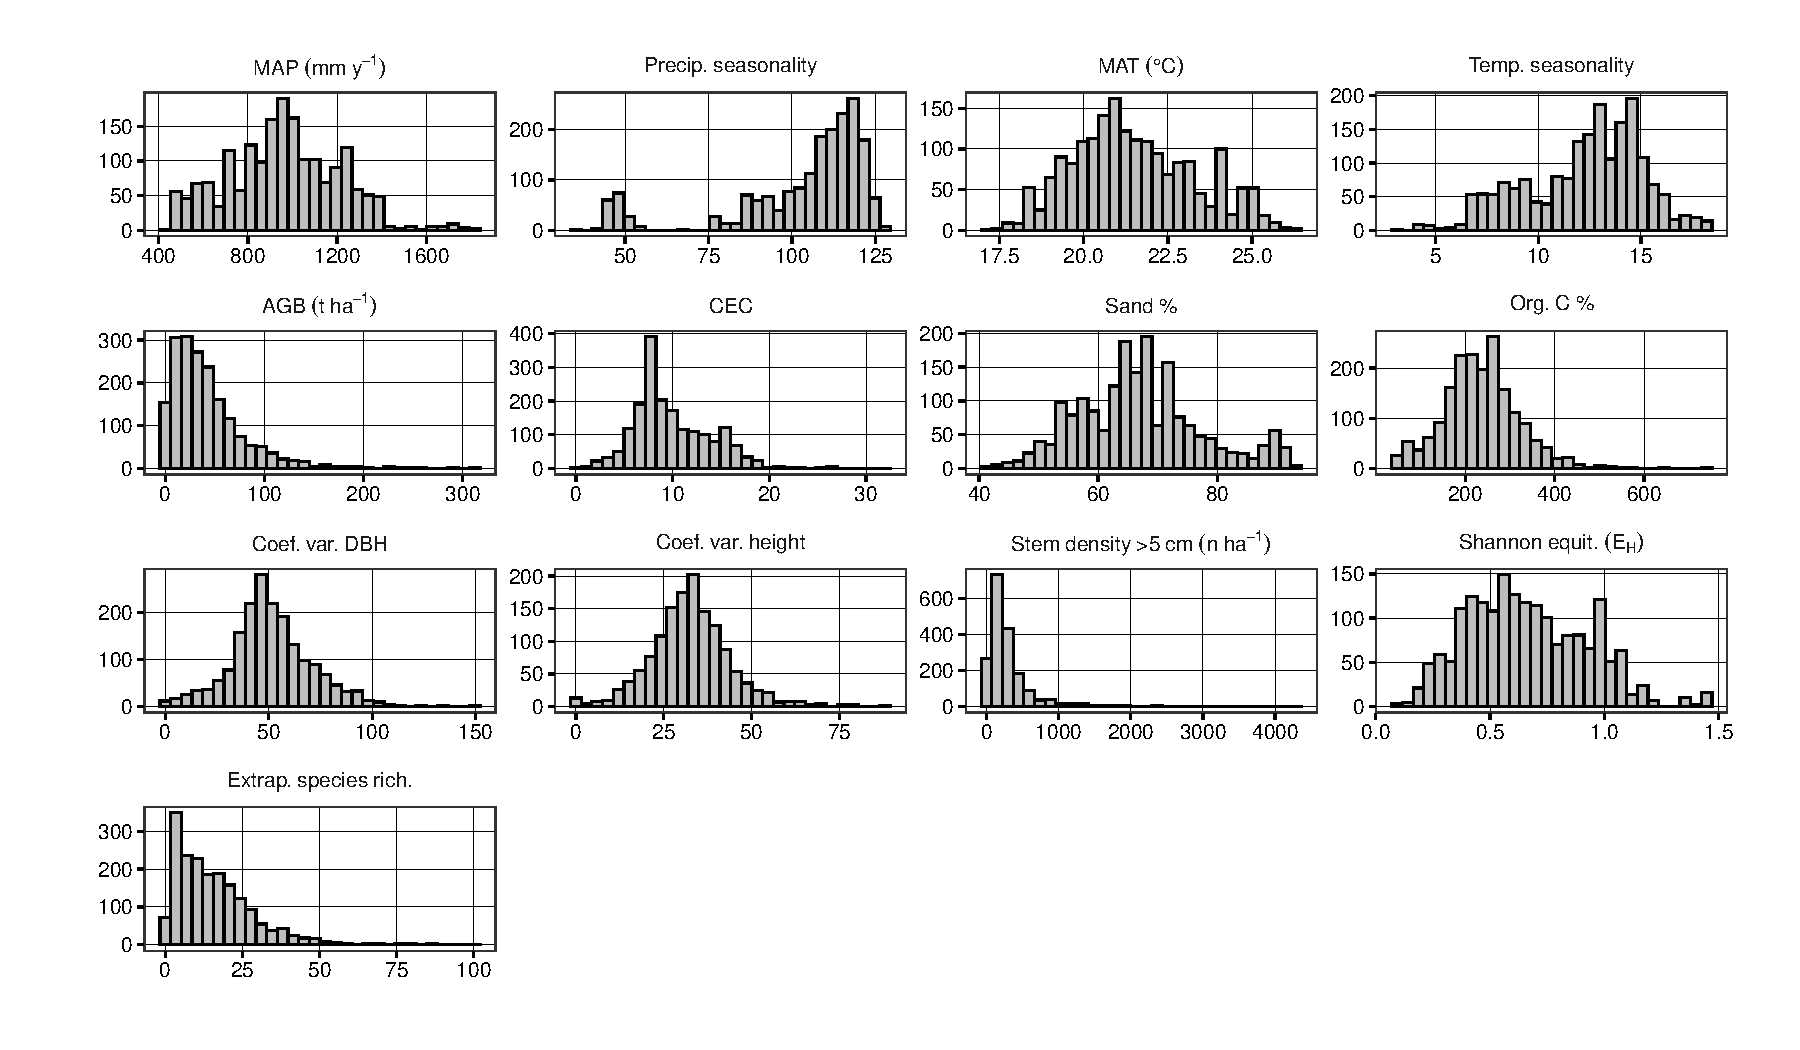
\includegraphics[width=\textwidth]{histogram_raw_obs}
	\caption{Histograms of raw untransformed observed variables used in final analyses.}
	\label{histogram_raw_obs}
\end{figure}

\begin{figure}[H]
\centering
	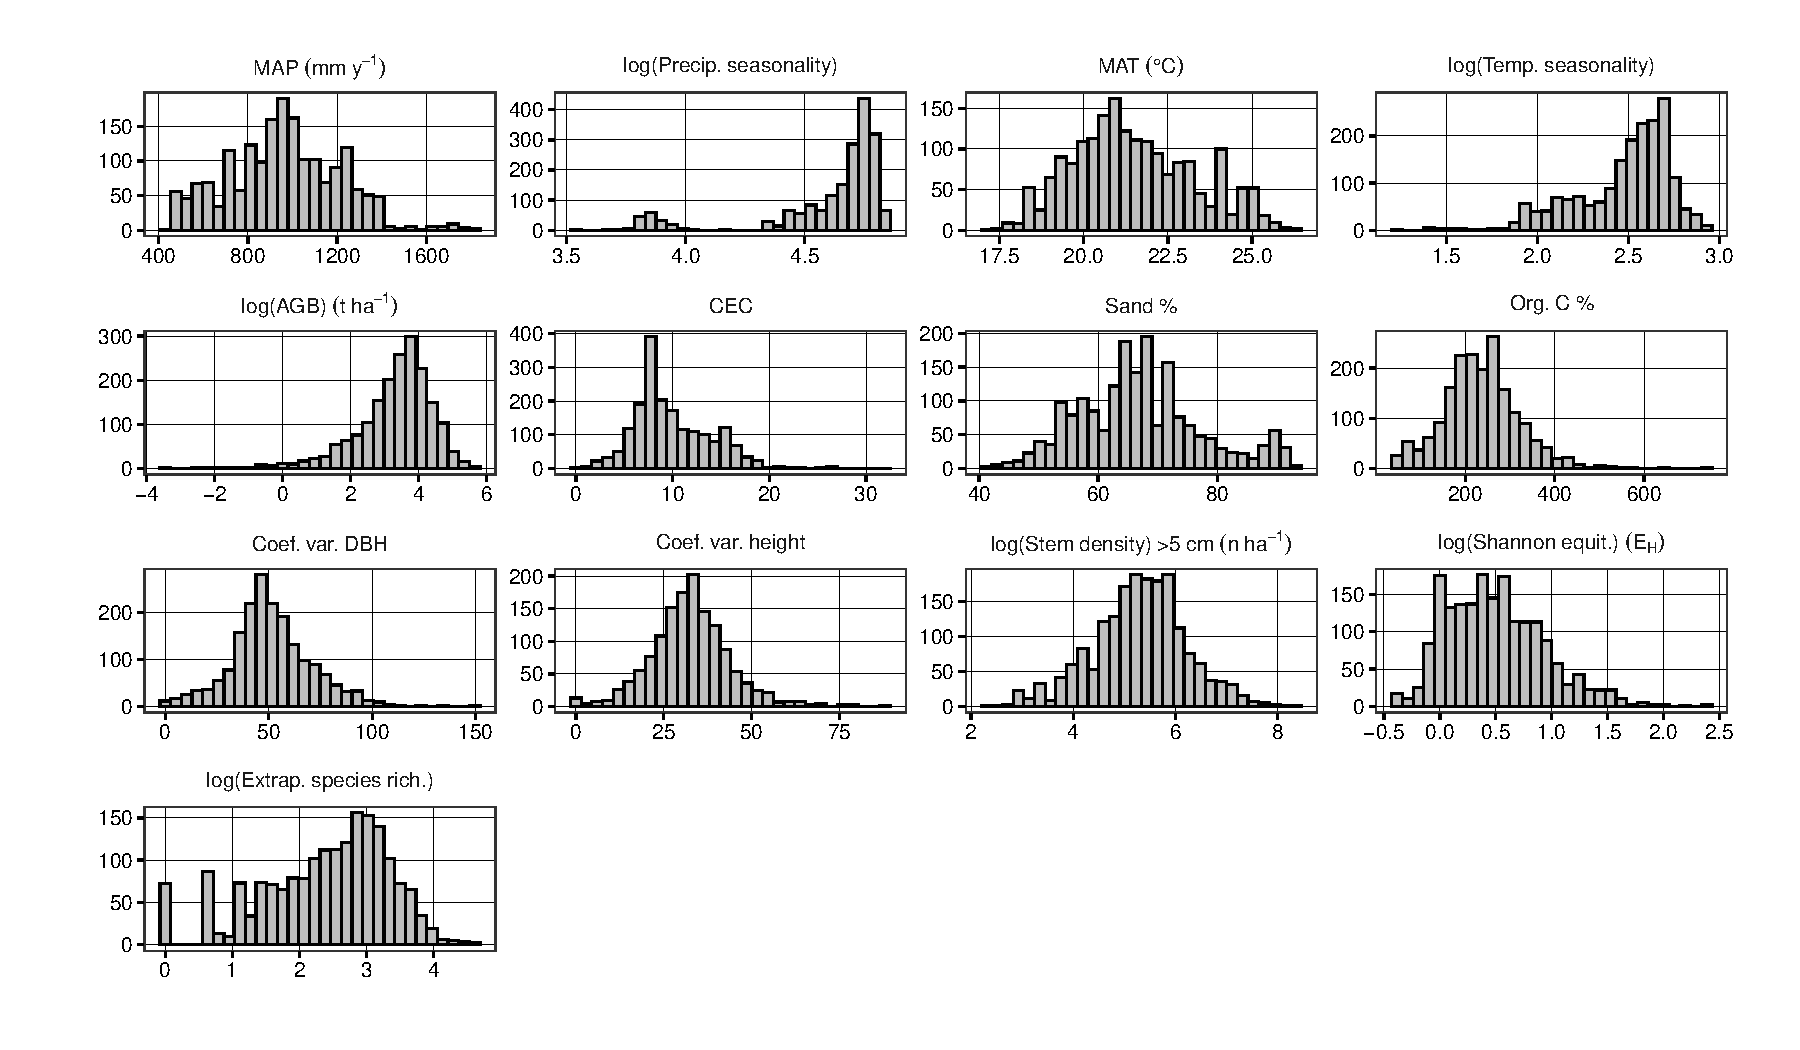
\includegraphics[width=\textwidth]{histogram_trans_obs}
	\caption{Histograms of observed variables transformed to achieve a normal frequency distribution.}
	\label{histogram_trans_obs}
\end{figure}

\section*{Appendix 4 - Table of correlation fit statistics} \label{appendixd}


% Table created by stargazer v.5.2.2 by Marek Hlavac, Harvard University. E-mail: hlavac at fas.harvard.edu
% Date and time: Wed, Jun 24, 2020 - 13:33:02
\begin{table}[!htbp] \centering 
  \caption{} 
  \label{corr_ci_tab} 
\begin{tabular}{@{\extracolsep{5pt}} ccccccc} 
\\[-1.8ex]\hline 
\hline \\[-1.8ex] 
x\_var & y\_var & raw.r & raw.lower & raw.upper & n & p \\ 
\hline \\[-1.8ex] 
Sand \% & Org. C (ppt) & $$-$0.620$ & $$-$0.650$ & $$-$0.580$ & $1235$ & p \textless 0.01 \\ 
Sand \% & CEC & $$-$0.510$ & $$-$0.550$ & $$-$0.470$ & $1235$ & p \textless 0.01 \\ 
Sand \% & MAP & $$-$0.500$ & $$-$0.540$ & $$-$0.460$ & $1235$ & p \textless 0.01 \\ 
Sand \% & PS & $0.350$ & $0.300$ & $0.400$ & $1235$ & p \textless 0.01 \\ 
Sand \% & MAT & $0.340$ & $0.280$ & $0.380$ & $1235$ & p \textless 0.01 \\ 
Sand \% & TS & $0.380$ & $0.330$ & $0.430$ & $1235$ & p \textless 0.01 \\ 
Sand \% & Sp. rich. & $$-$0.330$ & $$-$0.370$ & $$-$0.280$ & $1235$ & p \textless 0.01 \\ 
Sand \% & Shannon equit. & $0.250$ & $0.190$ & $0.300$ & $1235$ & p \textless 0.01 \\ 
Sand \% & Tree height CV & $$-$0.250$ & $$-$0.300$ & $$-$0.190$ & $981$ & p \textless 0.01 \\ 
Sand \% & DBH CV & $$-$0.170$ & $$-$0.230$ & $$-$0.120$ & $1233$ & p \textless 0.01 \\ 
Sand \% & Stems ha & $$-$0.100$ & $$-$0.160$ & $$-$0.050$ & $1235$ & p \textless 0.01 \\ 
Sand \% & AGB & $$-$0.270$ & $$-$0.320$ & $$-$0.220$ & $1235$ & p \textless 0.01 \\ 
Org. C (ppt) & CEC & $0.460$ & $0.410$ & $0.500$ & $1235$ & p \textless 0.01 \\ 
Org. C (ppt) & MAP & $0.440$ & $0.390$ & $0.480$ & $1235$ & p \textless 0.01 \\ 
Org. C (ppt) & PS & $$-$0.410$ & $$-$0.450$ & $$-$0.360$ & $1235$ & p \textless 0.01 \\ 
Org. C (ppt) & MAT & $$-$0.280$ & $$-$0.330$ & $$-$0.230$ & $1235$ & p \textless 0.01 \\ 
Org. C (ppt) & TS & $$-$0.280$ & $$-$0.330$ & $$-$0.230$ & $1235$ & p \textless 0.01 \\ 
Org. C (ppt) & Sp. rich. & $0.150$ & $0.090$ & $0.200$ & $1235$ & p \textless 0.01 \\ 
Org. C (ppt) & Shannon equit. & $$-$0.160$ & $$-$0.220$ & $$-$0.110$ & $1235$ & p \textless 0.01 \\ 
Org. C (ppt) & Tree height CV & $0.180$ & $0.120$ & $0.240$ & $981$ & p \textless 0.01 \\ 
Org. C (ppt) & DBH CV & $0.140$ & $0.080$ & $0.190$ & $1233$ & p \textless 0.01 \\ 
Org. C (ppt) & Stems ha & $0.090$ & $0.030$ & $0.140$ & $1235$ & p \textless 0.01 \\ 
Org. C (ppt) & AGB & $0.270$ & $0.220$ & $0.320$ & $1235$ & p \textless 0.01 \\ 
CEC & MAP & $$-$0.070$ & $$-$0.130$ & $$-$0.020$ & $1235$ & p \textless 0.01 \\ 
CEC & PS & $$-$0.590$ & $$-$0.630$ & $$-$0.550$ & $1235$ & p \textless 0.01 \\ 
CEC & MAT & $0.170$ & $0.120$ & $0.220$ & $1235$ & p \textless 0.01 \\ 
CEC & TS & $0.070$ & $0.010$ & $0.120$ & $1235$ & p \textless 0.05 \\ 
CEC & Sp. rich. & $$-$0.100$ & $$-$0.160$ & $$-$0.050$ & $1235$ & p \textless 0.01 \\ 
CEC & Shannon equit. & $$-$0.120$ & $$-$0.180$ & $$-$0.070$ & $1235$ & p \textless 0.01 \\ 
CEC & Tree height CV & $0.090$ & $0.020$ & $0.150$ & $981$ & p \textless 0.01 \\ 
CEC & DBH CV & $0.130$ & $0.080$ & $0.190$ & $1233$ & p \textless 0.01 \\ 
CEC & Stems ha & $$-$0.090$ & $$-$0.140$ & $$-$0.030$ & $1235$ & p \textless 0.01 \\ 
CEC & AGB & $0.080$ & $0.030$ & $0.140$ & $1235$ & p \textless 0.01 \\ 
MAP & PS & $$-$0.070$ & $$-$0.130$ & $$-$0.020$ & $1235$ & p \textless 0.05 \\ 
MAP & MAT & $$-$0.200$ & $$-$0.260$ & $$-$0.150$ & $1235$ & p \textless 0.01 \\ 
MAP & TS & $$-$0.770$ & $$-$0.790$ & $$-$0.740$ & $1235$ & p \textless 0.01 \\ 
MAP & Sp. rich. & $0.400$ & $0.350$ & $0.450$ & $1235$ & p \textless 0.01 \\ 
MAP & Shannon equit. & $$-$0.130$ & $$-$0.180$ & $$-$0.070$ & $1235$ & p \textless 0.01 \\ 
MAP & Tree height CV & $0.250$ & $0.190$ & $0.310$ & $981$ & p \textless 0.01 \\ 
MAP & DBH CV & $0.120$ & $0.060$ & $0.170$ & $1233$ & p \textless 0.01 \\ 
MAP & Stems ha & $0.070$ & $0.010$ & $0.120$ & $1235$ & p \textless 0.05 \\ 
MAP & AGB & $0.230$ & $0.180$ & $0.280$ & $1235$ & p \textless 0.01 \\ 
precip\_seas\_std & MAT & $0$ & $$-$0.050$ & $0.060$ & $1235$ & p = 0.95 \\ 
precip\_seas\_std & TS & $0.140$ & $0.080$ & $0.190$ & $1235$ & p \textless 0.01 \\ 
precip\_seas\_std & Sp. rich. & $0.130$ & $0.070$ & $0.180$ & $1235$ & p \textless 0.01 \\ 
precip\_seas\_std & Shannon equit. & $0.070$ & $0.010$ & $0.130$ & $1235$ & p \textless 0.05 \\ 
precip\_seas\_std & Tree height CV & $$-$0.060$ & $$-$0.120$ & $0.010$ & $981$ & p = 0.07 \\ 
precip\_seas\_std & DBH CV & $$-$0.100$ & $$-$0.150$ & $$-$0.040$ & $1233$ & p \textless 0.01 \\ 
precip\_seas\_std & Stems ha & $$-$0.030$ & $$-$0.080$ & $0.030$ & $1235$ & p = 0.33 \\ 
precip\_seas\_std & AGB & $$-$0.190$ & $$-$0.240$ & $$-$0.130$ & $1235$ & p \textless 0.01 \\ 
MAT & TS & $0.060$ & $0$ & $0.120$ & $1235$ & p \textless 0.05 \\ 
MAT & Sp. rich. & $$-$0.170$ & $$-$0.220$ & $$-$0.120$ & $1235$ & p \textless 0.01 \\ 
MAT & Shannon equit. & $0$ & $$-$0.060$ & $0.060$ & $1235$ & p = 0.98 \\ 
MAT & Tree height CV & $$-$0.040$ & $$-$0.100$ & $0.020$ & $981$ & p = 0.2 \\ 
MAT & DBH CV & $0.060$ & $0.010$ & $0.120$ & $1233$ & p \textless 0.05 \\ 
MAT & Stems ha & $$-$0.150$ & $$-$0.210$ & $$-$0.100$ & $1235$ & p \textless 0.01 \\ 
MAT & AGB & $$-$0.090$ & $$-$0.150$ & $$-$0.040$ & $1235$ & p \textless 0.01 \\ 
TS & Sp. rich. & $$-$0.440$ & $$-$0.480$ & $$-$0.390$ & $1235$ & p \textless 0.01 \\ 
TS & Shannon equit. & $0.200$ & $0.150$ & $0.250$ & $1235$ & p \textless 0.01 \\ 
TS & Tree height CV & $$-$0.210$ & $$-$0.270$ & $$-$0.150$ & $981$ & p \textless 0.01 \\ 
TS & DBH CV & $$-$0.090$ & $$-$0.150$ & $$-$0.040$ & $1233$ & p \textless 0.01 \\ 
TS & Stems ha & $$-$0.050$ & $$-$0.110$ & $0.010$ & $1235$ & p = 0.08 \\ 
TS & AGB & $$-$0.180$ & $$-$0.230$ & $$-$0.120$ & $1235$ & p \textless 0.01 \\ 
Sp. rich. & Shannon equit. & $$-$0.580$ & $$-$0.620$ & $$-$0.540$ & $1235$ & p \textless 0.01 \\ 
Sp. rich. & Tree height CV & $0.300$ & $0.250$ & $0.360$ & $981$ & p \textless 0.01 \\ 
Sp. rich. & DBH CV & $0.300$ & $0.250$ & $0.350$ & $1233$ & p \textless 0.01 \\ 
Sp. rich. & Stems ha & $0.240$ & $0.190$ & $0.300$ & $1235$ & p \textless 0.01 \\ 
Sp. rich. & AGB & $0.310$ & $0.260$ & $0.360$ & $1235$ & p \textless 0.01 \\ 
Shannon equit. & Tree height CV & $$-$0.120$ & $$-$0.190$ & $$-$0.060$ & $981$ & p \textless 0.01 \\ 
Shannon equit. & DBH CV & $$-$0.200$ & $$-$0.250$ & $$-$0.140$ & $1233$ & p \textless 0.01 \\ 
Shannon equit. & Stems ha & $$-$0.410$ & $$-$0.460$ & $$-$0.360$ & $1235$ & p \textless 0.01 \\ 
Shannon equit. & AGB & $$-$0.350$ & $$-$0.400$ & $$-$0.300$ & $1235$ & p \textless 0.01 \\ 
Tree height CV & DBH CV & $0.470$ & $0.420$ & $0.520$ & $981$ & p \textless 0.01 \\ 
Tree height CV & Stems ha & $0.010$ & $$-$0.060$ & $0.070$ & $981$ & p = 0.86 \\ 
Tree height CV & AGB & $0.240$ & $0.180$ & $0.290$ & $981$ & p \textless 0.01 \\ 
DBH CV & Stems ha & $0.110$ & $0.060$ & $0.170$ & $1233$ & p \textless 0.01 \\ 
DBH CV & AGB & $0.430$ & $0.390$ & $0.480$ & $1233$ & p \textless 0.01 \\ 
Stems ha & AGB & $0.590$ & $0.550$ & $0.620$ & $1235$ & p \textless 0.01 \\ 
\hline \\[-1.8ex] 
\end{tabular} 
\end{table} 


\end{document}


% https://jslefche.github.io/sem_book/coefficients.html

